\section{Radionuclide Transport Validation}\label{sec:nuclide_benchmarks}

As described in Section \ref{sec:nuclide_models}, hydrologic contaminant 
transport in \Cyder is implemented with four interchangeable  methods in a 
modular software design. These modeling options alternately optimize speed and 
fidelity in representations of barrier components within the repository concept 
(i.e. waste form, waste package, buffer, and geologic medium)\cite{huff_hydrologic_2013}.  Simplistic models include a congruent 
release component degradation rate model and a mixed cell control volume model. For 
systems in which the flow can be assumed constant, a medium fidelity lumped 
parameter dispersion model is implemented. Also implemented is a Brenner 
approximation to the Leij et al.  solution to the advection dispersion equation 
for Cauchy boundary condition \cite{brenner_diffusion_1962, 
leij_analytical_1991, van_genuchten_analytical_1982}.  

Analyses in Table \ref{tab:nuclide_bench_tab} were conducted to compare the 
performance of these radionuclide transport models with more detailed results from the 
Clay \gls{GDSE}. 


\begin{table}[ht!]
\centering
\footnotesize{
  \begin{tabularx}{\textwidth}{|X|l|l|r|}
\multicolumn{4}{c}{\textbf{Radionuclide Transport Benchmark Cases}}\\
\hline
\textbf{Parameter} & \textbf{Symbol} & \textbf{Units} & \textbf{Value Range} \\
\hline
Hydraulic & & & \\
Reference & & & \\
Diffusivity& $\alpha_{h,ref}$& $[m^2s]$ & $10^{-15} - 10^{-8}$ \\
\hline
Hydraulic & & & \\
Conductivity& $K_{h}$& $[m \cdot s^{-1}]$ & $10^{-13} - 10^{-3}$ \\
\hline
Advective  & & & \\
Water & & & \\
Velocity & $v_{adv}$ & $[m\cdot s^{-1}]$ & $2\times10^{-16}-2\times10^{-12}$ \\
\hline
Sorption \& & & & Reducing - \\
Behavior & $K_{d,i}$& $[m^3\cdot kg^{-1}]$ & Oxidizing \\
\hline
Solubility &  & & Reducing -\\
Limitation & $C_{sol,i}$ & $[kg\cdot m^{-3}3]$& Oxidizing \\
\hline
WF& & & \\
Degradation& & & \\
Rate& $f_{wf}$ & [month$^{-1}$]& $0.0001-0.9$ \\
\hline
\end{tabularx}
\caption{The sensitivity analyses conducted in this work covered a range of 
thermal and hydrologic parameters in the context of canonical fuel cycle choices.}
}
\label{tab:nuclide_bench_tab}
\end{table}




%\subsection{Case I : Diffusion Coefficient and Inventory Sensitivity}
%

\subsubsection{Sensitivity to Diffusion and Contaminant Inventory GDSM Results}

In the parametric sensitivity analysis discussed in section
\ref{sec:diffusivity}, it was shown that
the peak doses due to highly soluble, non-sorbing elements such as $I$ and $Cl$, 
are  proportional to the radionuclide inventory and 
largely directly proportional to the relative diffusivity. This can be seen for 
the cases of $^{129}I$ and $^{36}Cl$ in Figures \ref{fig:DCInvI129}, 
\ref{fig:DCInvI129MF}, \ref{fig:DCInvCl36} and \ref{fig:DCInvCl36MF}.

\begin{figure}[ht]
\centering
\begin{minipage}[b]{0.45\linewidth}

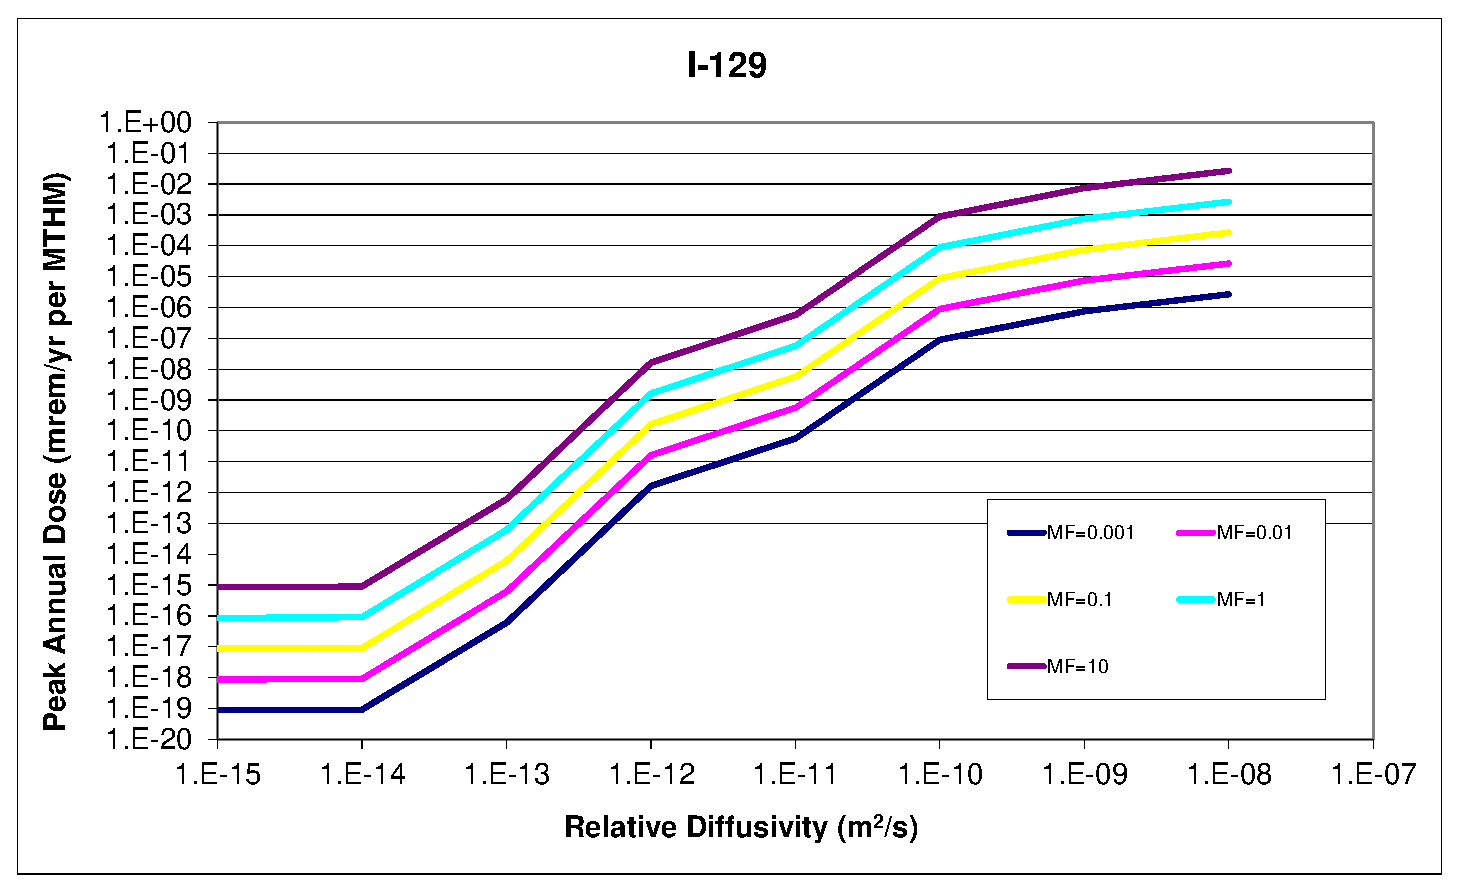
\includegraphics[width=\linewidth]{./chapters/nuclide_sensitivity/clay/DiffCoeffAndInvEBSFail/I-129.eps}
\caption{$^{129}I$ relative diffusivity sensitivity.}
\label{fig:DCInvI129}

\end{minipage}
\hspace{0.05\linewidth}
\begin{minipage}[b]{0.45\linewidth}

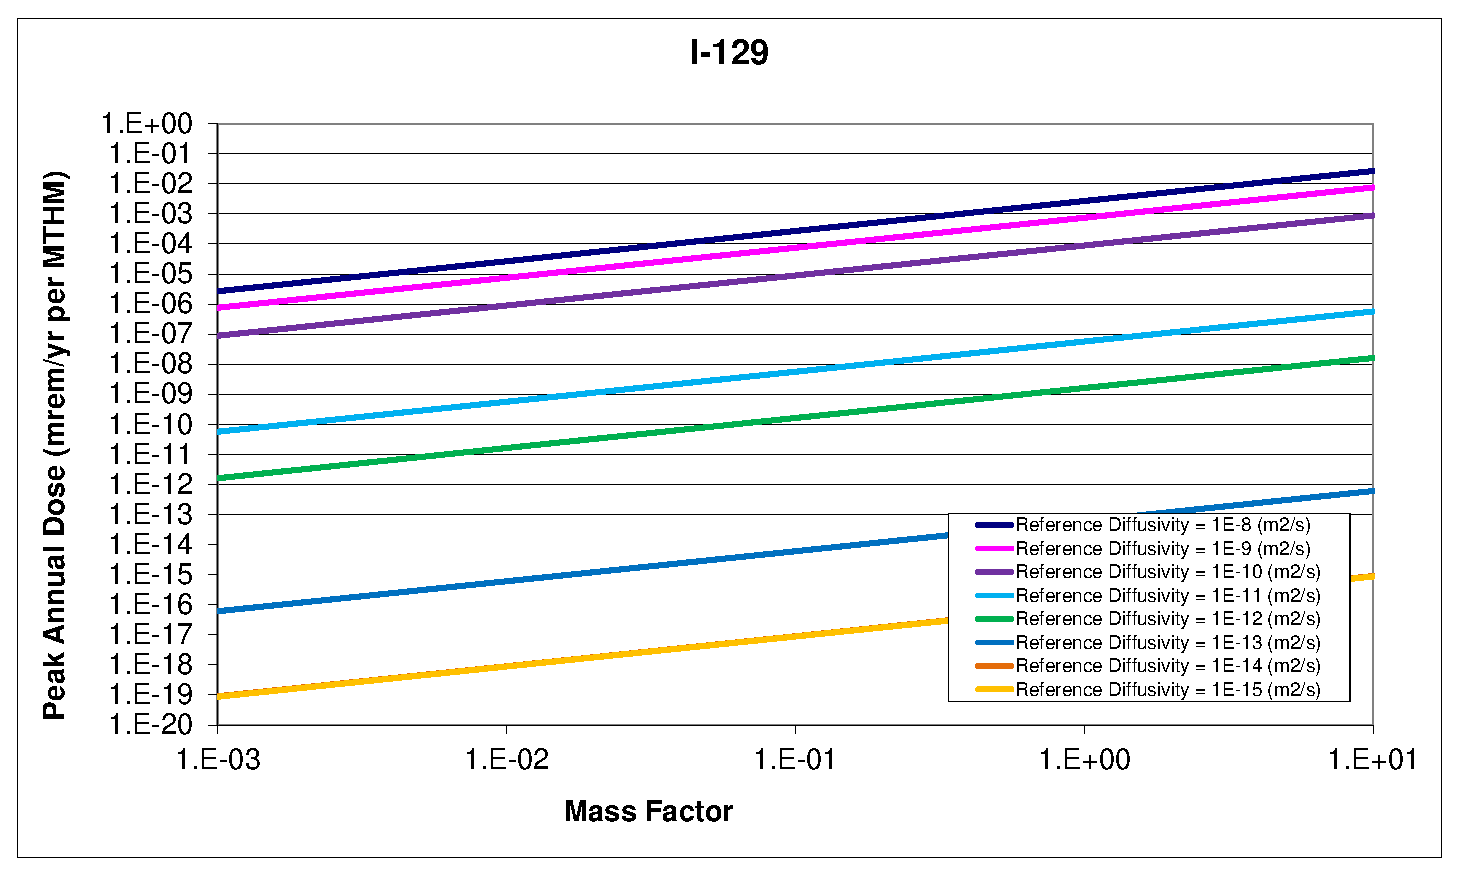
\includegraphics[width=\linewidth]{./chapters/nuclide_sensitivity/clay/DiffCoeffAndInvEBSFail/I-129-MF.eps}
\caption{$^{129}I$ mass factor sensitivity.}
\label{fig:DCInvI129MF}

\end{minipage}
\end{figure}

\begin{figure}[ht]
\begin{minipage}[b]{0.45\linewidth}

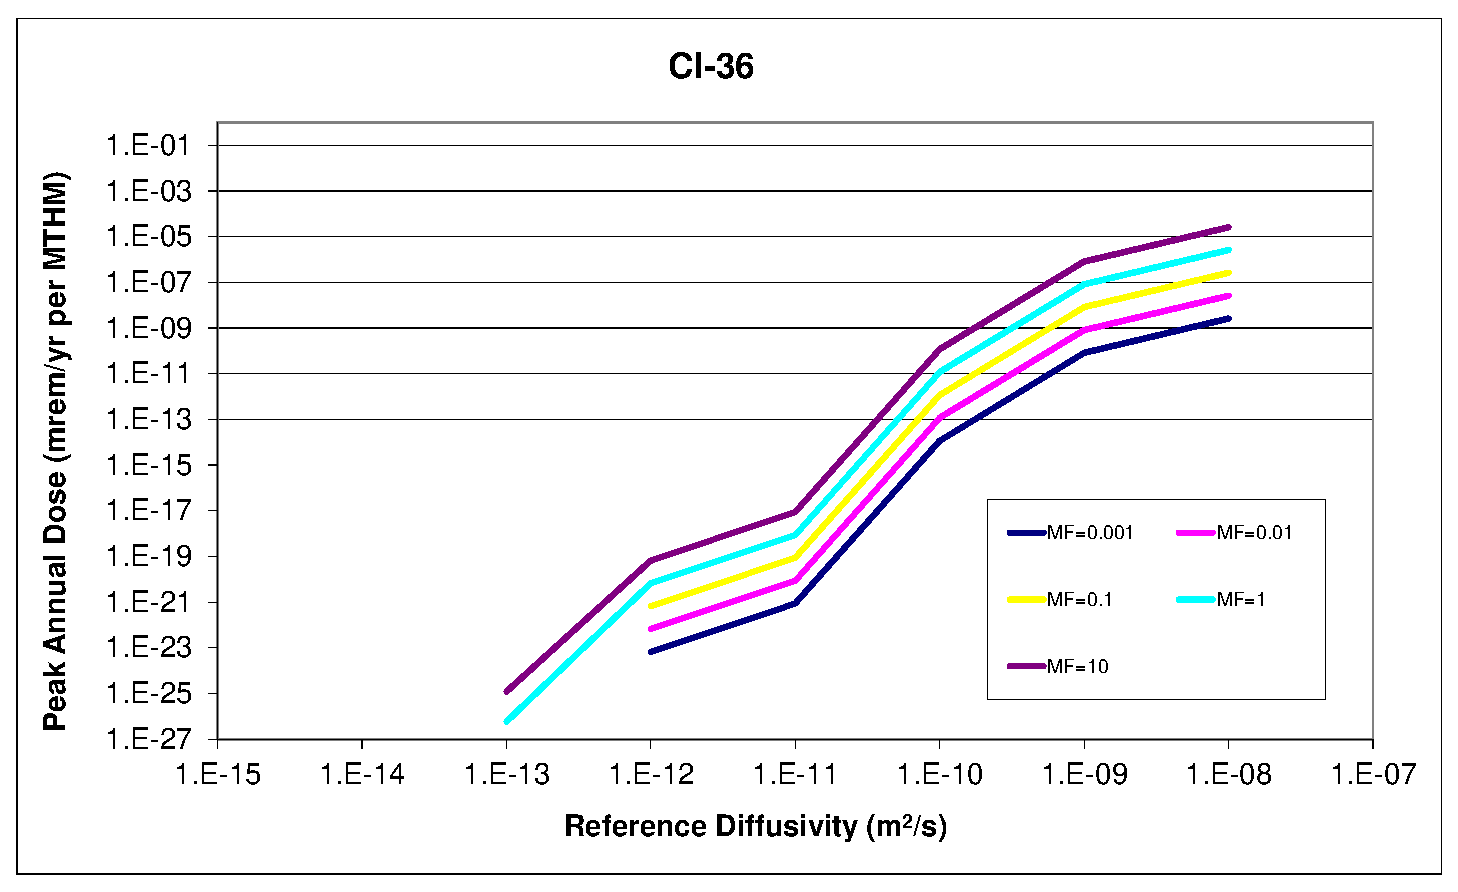
\includegraphics[width=\linewidth]{./chapters/nuclide_sensitivity/clay/DiffCoeffAndInvEBSFail/Cl-36.eps}
\caption{$^{36}Cl$ relative diffusivity sensitivity.}
\label{fig:DCInvCl36}

\end{minipage}
\hspace{0.05\linewidth}
\begin{minipage}[b]{0.45\linewidth}

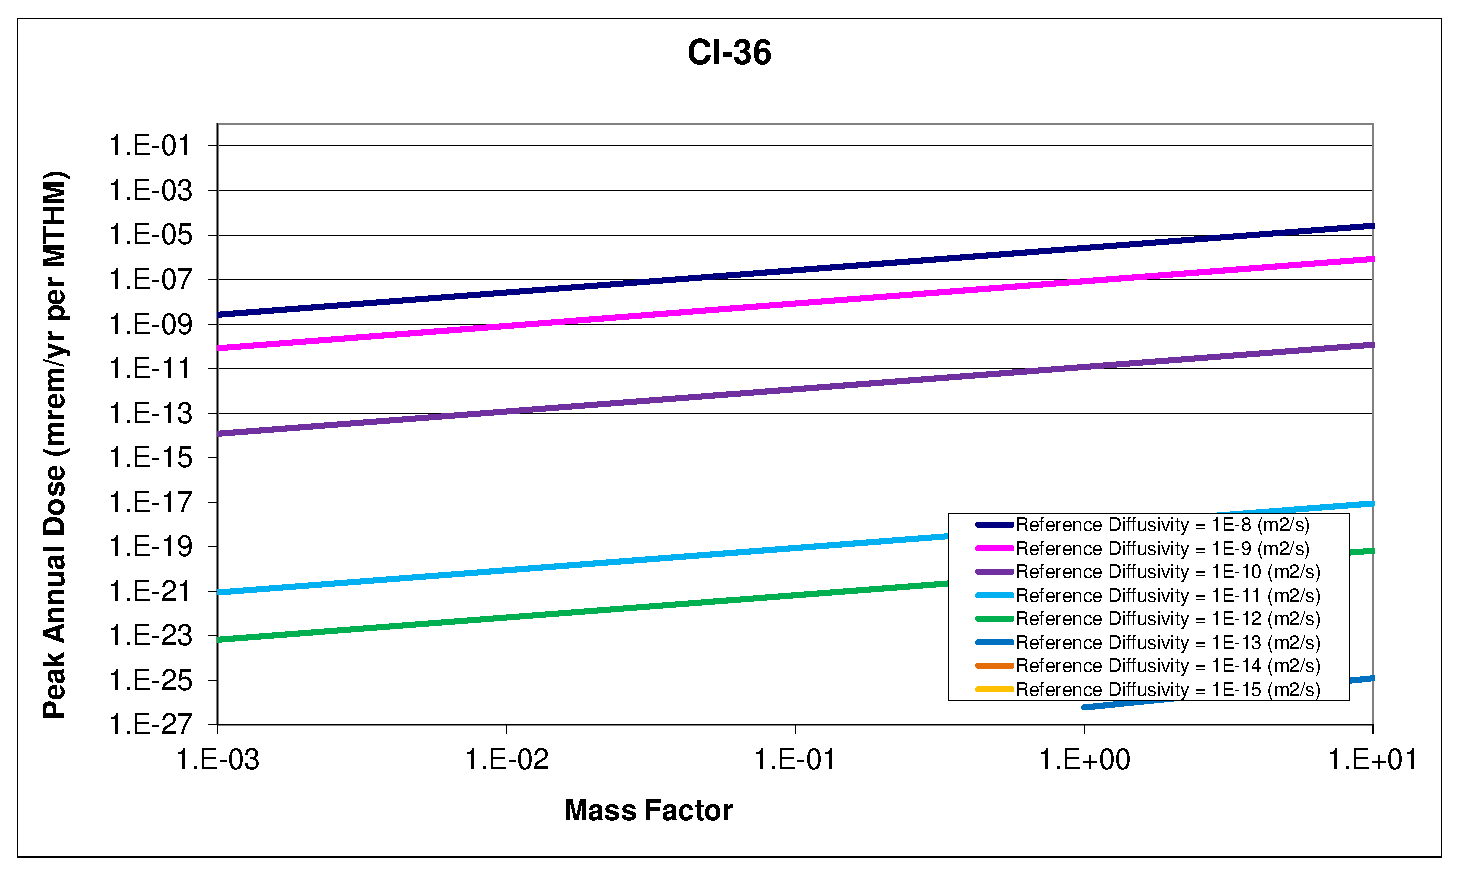
\includegraphics[width=\linewidth]{./chapters/nuclide_sensitivity/clay/DiffCoeffAndInvEBSFail/Cl-36-MF.eps}
\caption{$^{36}Cl$ mass factor sensitivity.}
\label{fig:DCInvCl36MF}

\end{minipage}
\end{figure}

Long lived $^{129}I$ and $^{36}Cl$ are assumed to have near complete solubility, 
so in Figures \ref{fig:DCInvI129} and \ref{fig:DCInvCl36}, the effect of a 
solubility limited attenuation regime is not seen. Even for very low 
diffusivities, the diffusion length of the far field is the primary barrier. In 
Figures \ref{fig:DCInvI129MF} and \ref{fig:DCInvCl36MF} it is clear that in the 
absence of solubility limitation and sorption, the peak dose is directly 
proportional to mass factor. 

Both $Cl$ and $I$ are soluble and non-sorbing. The amount of $^{129}I$ in the 
\gls{SNF} inventory is greater than the amount of $^{36}Cl$, so a difference in 
magnitudes are expected, however, the trends should be the same. Since the 
halflife of $^{36}Cl$, $3\times10^5[yr]$, is much shorter than the half life of 
$^{129}I$, $1.6\times10^7[yr]$, a stronger proportional dependence on mass 
factor is seen for $Cl$ due to its higher decay rate. 

With the exception of those dose-contributors assumed to be completely soluble, 
two regimes were visible in the results of this analysis. In low diffusion 
coefficient regime, the diffusive pathway through the homogeneous permeable 
porous medium in the far field continues to be a  dominant barrier to nuclide 
release for normal (non-intrusive) repository conditions. 

In the second regime, for very high diffusion coefficients, the effects of 
additional attenuation phenomena in the natural system can be seen.  The 
dependence of peak annual dose on mass factor was consistently directly 
proportional for all isotopic groups.

The peak doses due to solubility limited, sorbing elements such as $Np$ and 
$Tc$ demonstrate two major regimes. In the first regime, for 
low values of mass factor, the mean of the peak annual dose rates is directly 
proportional to both reference diffusivity and mass factor.  For higher values 
of mass factor, the sensitivity to reference diffusivity and mass factor are 
both attenuated at higher values.  The attenuation in these regimes 
is due to natural system attenuation, most notably, sorption.

$^{237}Np$ and $^{99}Tc$ exhibit a strong proportional relationship 
between diffusivity and dose in Figures \ref{fig:DCInvTc99} and 
\ref{fig:DCInvNp237}. This relationship is muted as diffusivity 
increases. Both are directly proportional to mass factor until they reach the 
point of attenuation by their solubility limits, as can be seen in 
Figures \ref{fig:DCInvTc99MF} and \ref{fig:DCInvNp237MF}.

\begin{figure}[ht!]
\centering
\begin{minipage}[b]{0.45\linewidth}
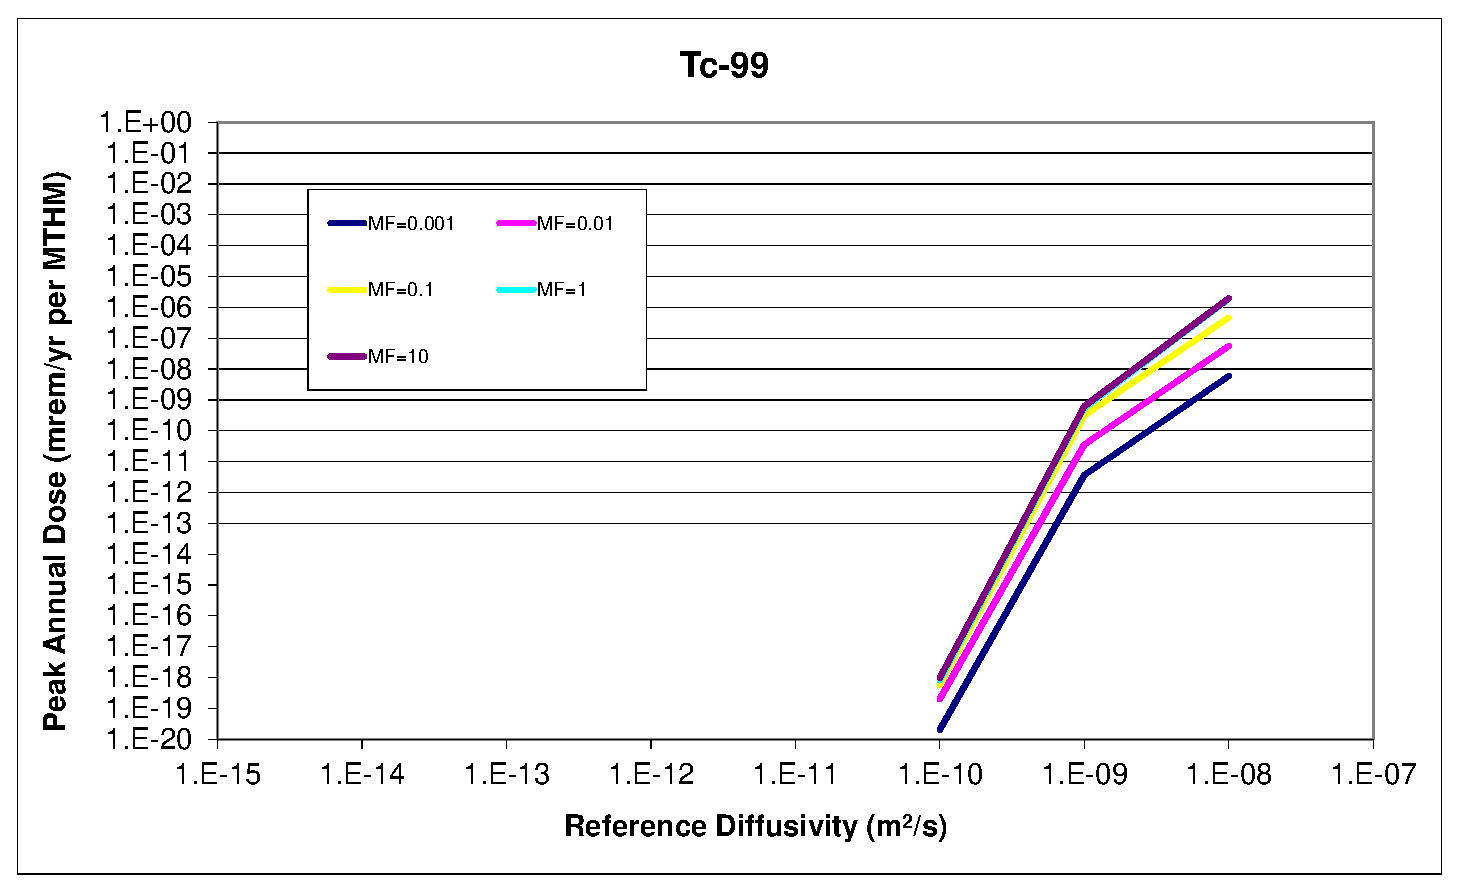
\includegraphics[width=\linewidth]{./chapters/nuclide_sensitivity/clay/DiffCoeffAndInvEBSFail/Tc-99.eps}
\caption{$^{99}Tc$ relative diffusivity sensitivity.} 
\label{fig:DCInvTc99}

\end{minipage}
\hspace{0.05\linewidth}
\begin{minipage}[b]{0.45\linewidth}

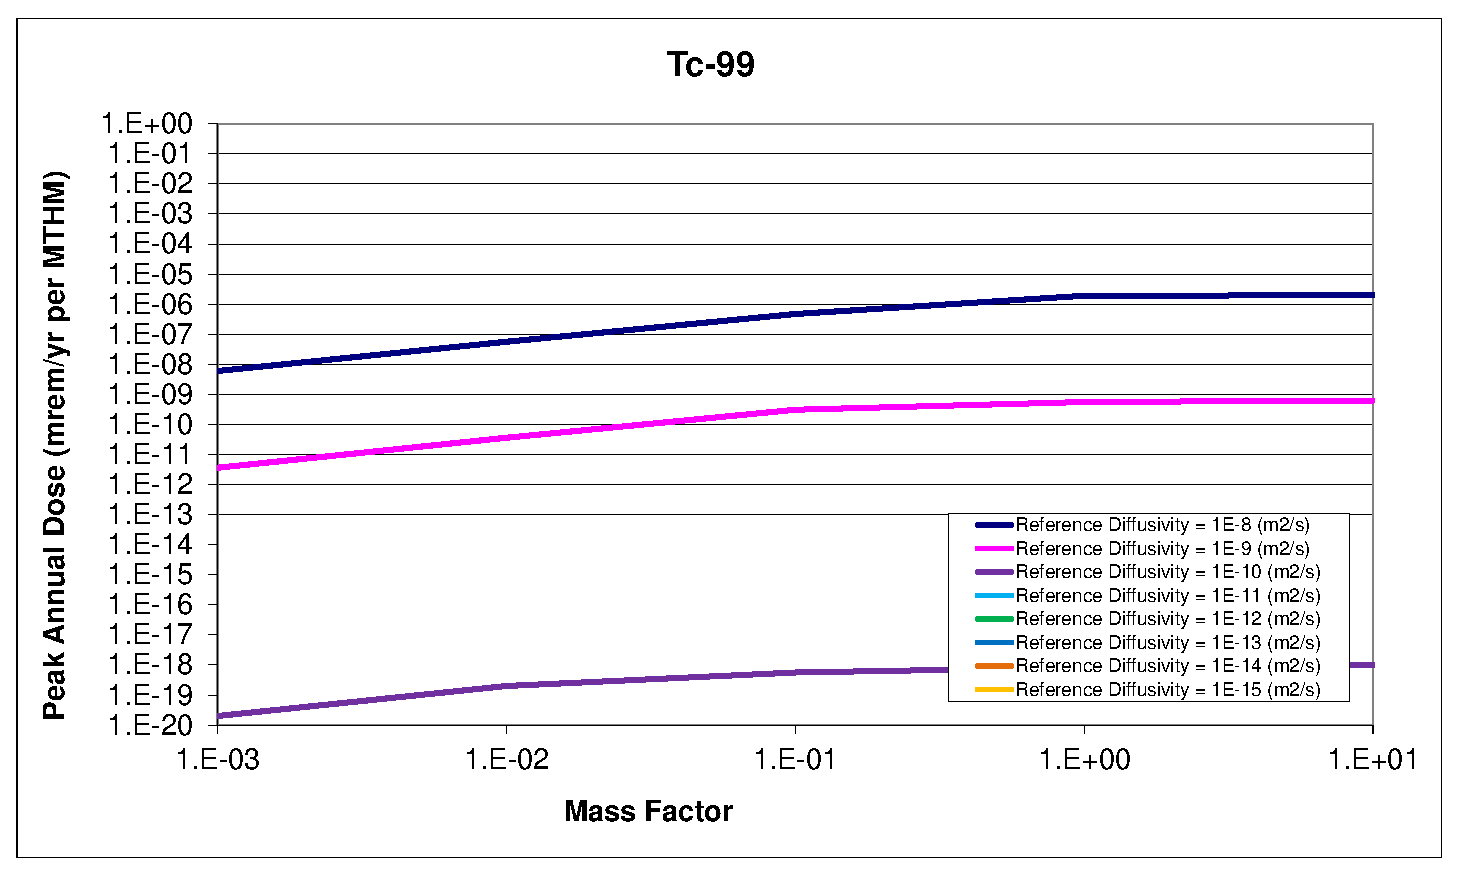
\includegraphics[width=\linewidth]{./chapters/nuclide_sensitivity/clay/DiffCoeffAndInvEBSFail/Tc-99-MF.eps}
\caption{$^{99}Tc$ mass factor sensitivity.}
\label{fig:DCInvTc99MF}

\end{minipage}
\end{figure}
\begin{figure}[ht]
\begin{minipage}[b]{0.45\linewidth}

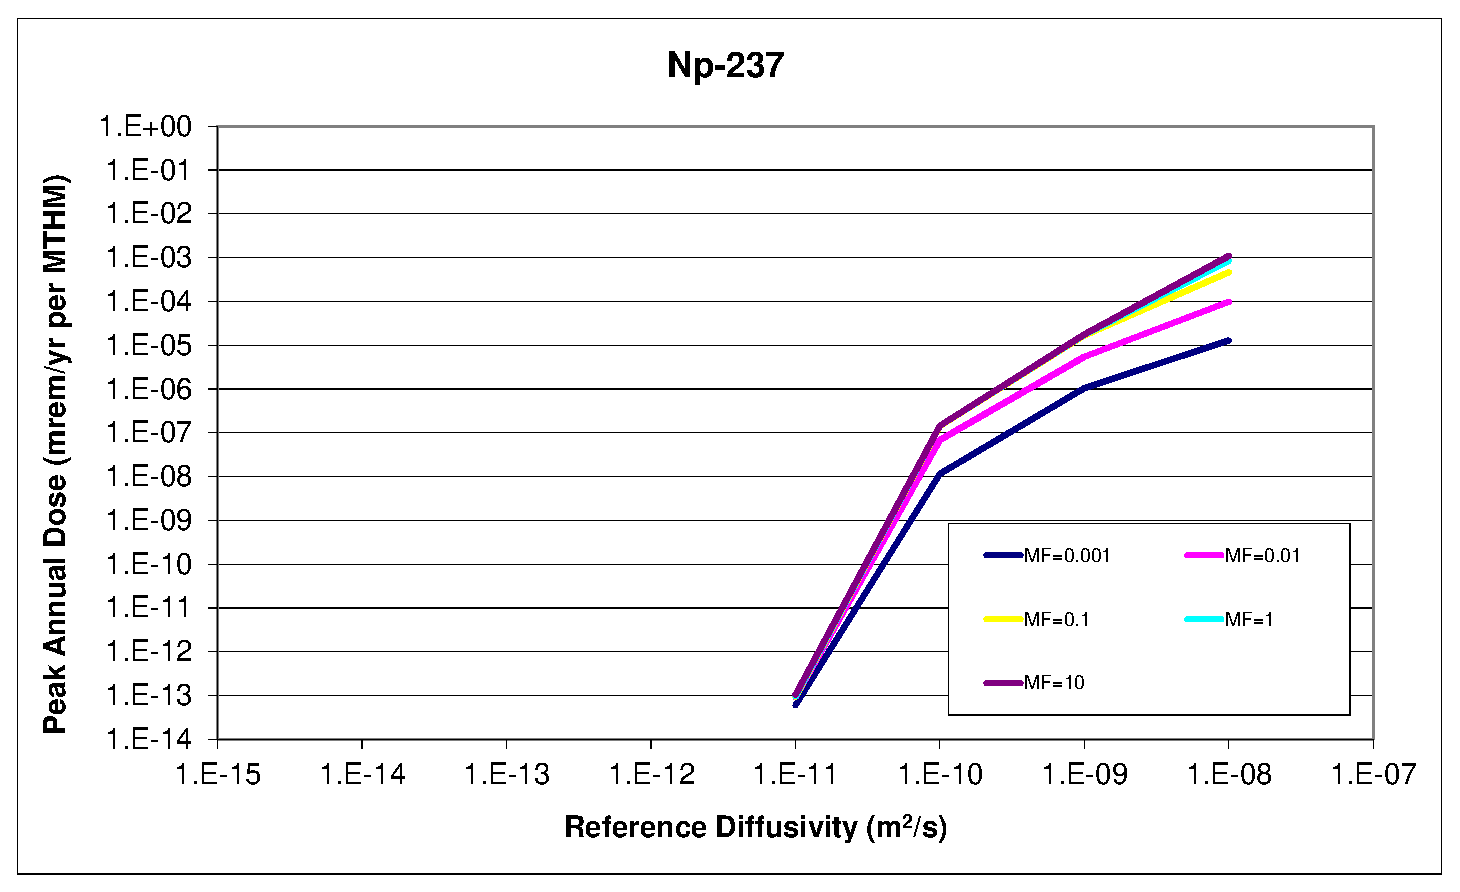
\includegraphics[width=\linewidth]{./chapters/nuclide_sensitivity/clay/DiffCoeffAndInvEBSFail/Np-237.eps}
\caption{$^{237}Np$ relative diffusivity sensitivity.} 
\label{fig:DCInvNp237}

\end{minipage}
\hspace{0.05\linewidth}
\begin{minipage}[b]{0.45\linewidth}

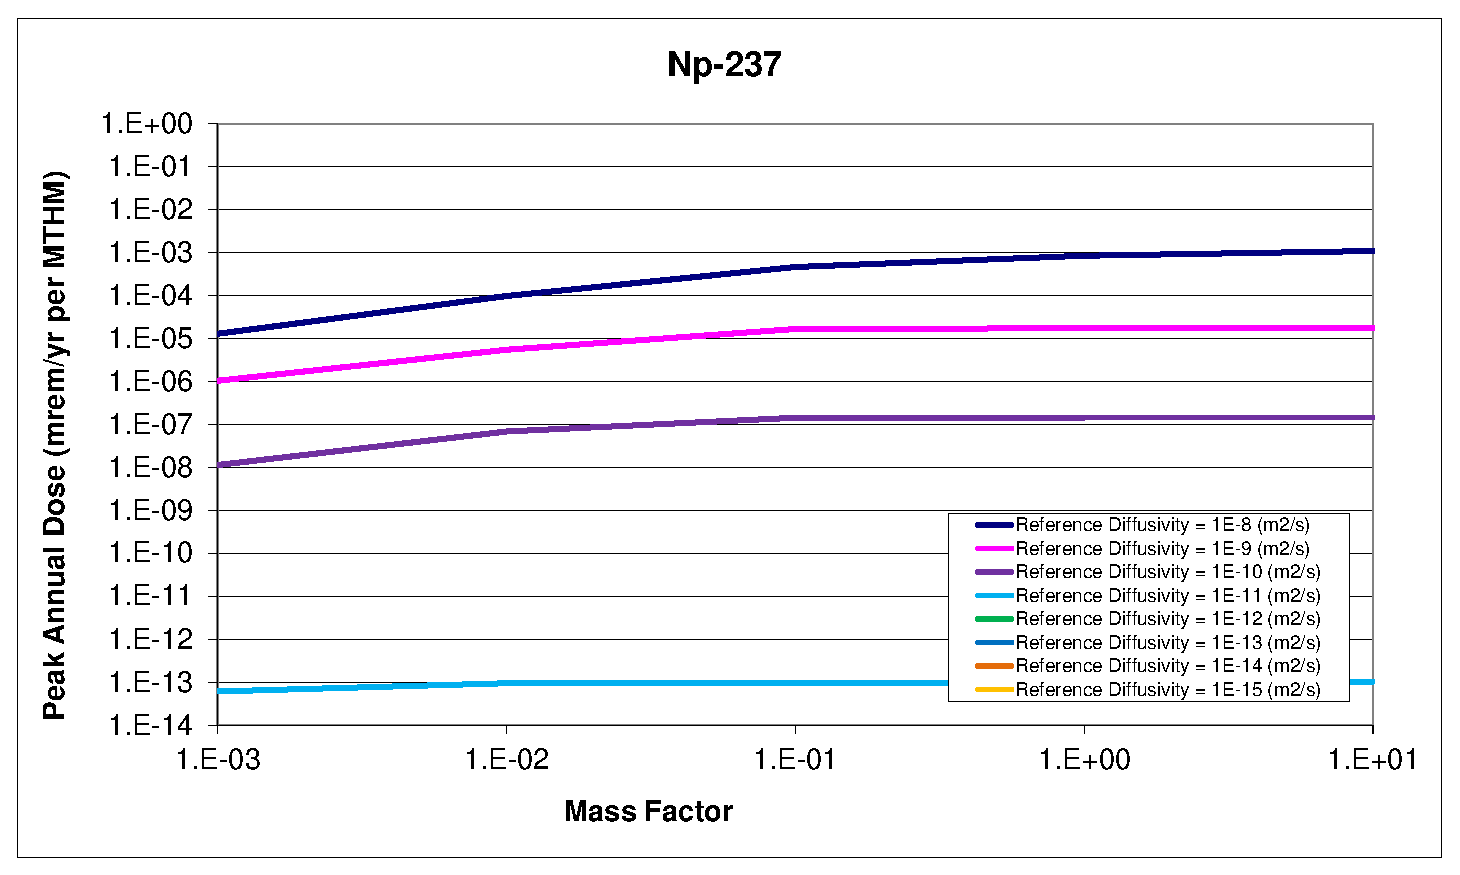
\includegraphics[width=\linewidth]{./chapters/nuclide_sensitivity/clay/DiffCoeffAndInvEBSFail/Np-237-MF.eps}
\caption{$^{237}Np$ mass factor sensitivity.}
\label{fig:DCInvNp237MF}

\end{minipage}
\end{figure}


\clearpage




\subsubsection{Sensitivity to Difussivity and Inventory Cyder Results}
A number of the radionuclide transport models in \Cyder depend on the diffusive 
characteristics of the medium. By evaluating the sensitivity to the reference 
diffusivity of the radionuclide transport in the MixedCell model, the 
the maximum releases due to isotopes treated as highly soluble and non-sorbing
were largely directly proportional to the relative diffusivity. 
This can be seen in Figure \ref{fig:mixed_diff} 
\begin{figure}[ht]
\centering
%\includegraphics[width=\linewidth]{./chapters/demonstration/bench/mixed_diff.eps}
\caption{Relative diffusivity sensitivity for a non-sorbing, infinitely soluble 
nuclide.}
\label{fig:DCInvI129}
\end{figure}


%\FloatBarrier
\subsection{Case I : Vertical Advective Velocity and Diffusion Coefficient Sensitivity}


\subsubsection{Advection vs. Diffusion Sensitivity GDSM Results}

In the parametric sensitivity analysis discussed in section
\ref{sec:AdvVelDiffCoeff}, it was shown that for isotopes of interest, higher
advective velocity and higher diffusivity lead to higher peak annual doses. 
However, the relationship between diffusivity and advective
velocity adds depth to the notion of a boundary between diffusive and advective
regimes.

The highly soluble and non-sorbing elements, $I$ and $Cl$ 
were expected to exhibit behavior that is highly sensitive 
to advection in the system in the advective regime but less sensitive to 
advection in the diffusive regime.  

In Figures \ref{fig:VAdvVelI129}, \ref{fig:VAdvVelI129VAdvVel}, 
\ref{fig:VAdvVelCl36}, and \ref{fig:VAdvVelCl36VAdvVel} , $^{129}I$ and 
$^{36}Cl$ are more sensitive to vertical advective velocity for lower vertical 
advective velocities. This demonstrates that for vertical advective velocities 
$6.31\times10^{-6}$ m/yr and above, lower reference diffusivities are 
ineffective at attenuating the mean of the peak doses for soluble, non-sorbing 
elements. 

\begin{figure}[htp!]
\begin{minipage}[b]{0.45\linewidth}
\centering
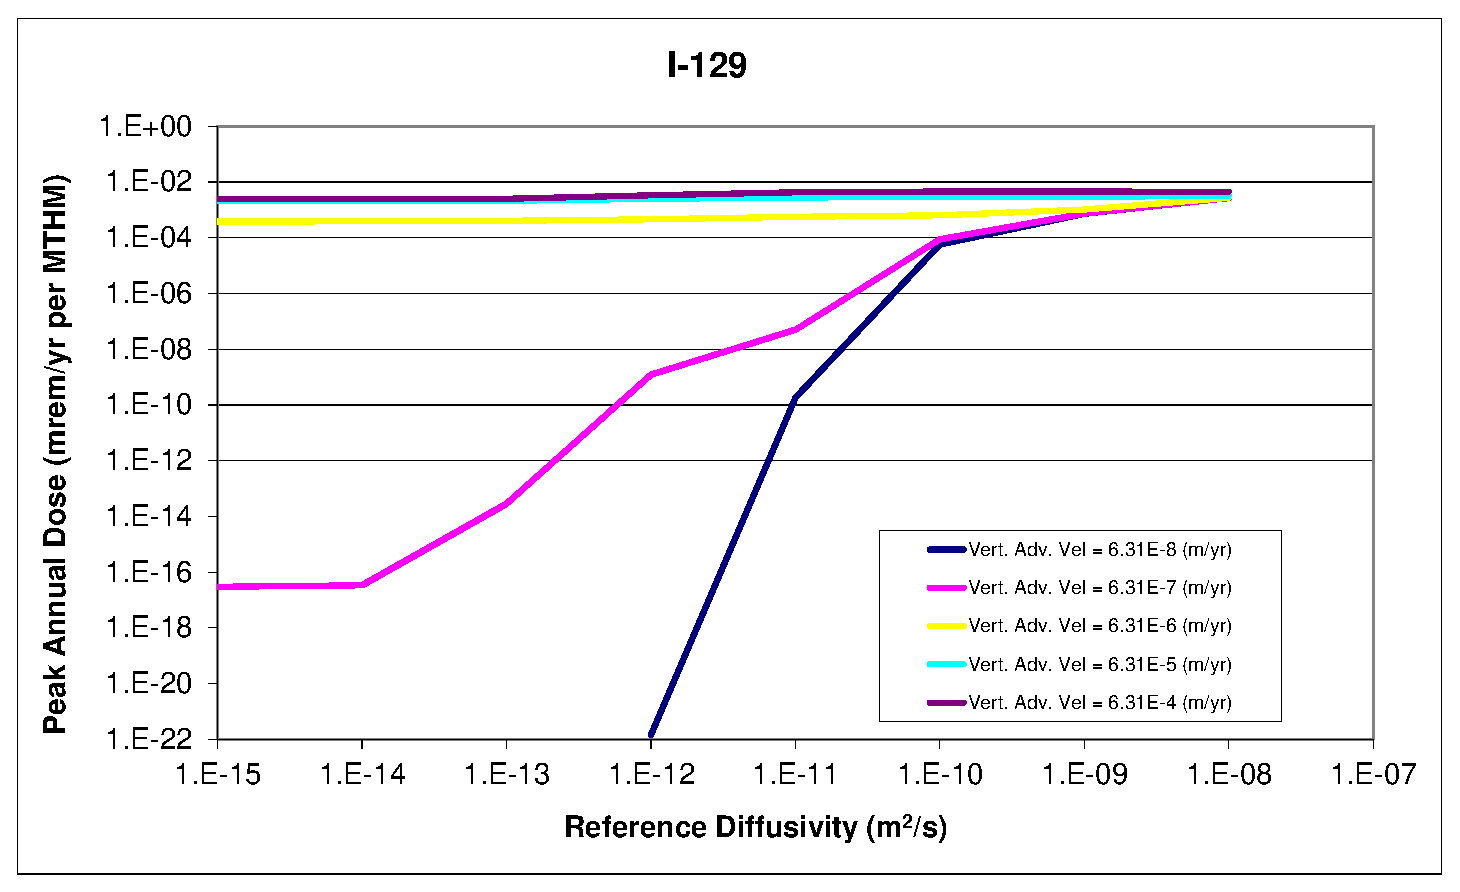
\includegraphics[width=\linewidth]{./chapters/nuclide_sensitivity/clay/AdvVelAndDiffCoeffEBSFail/I-129.eps}
\caption{$^{129}I$ reference diffusivity sensitivity.}
\label{fig:VAdvVelI129}

\end{minipage}
\hspace{0.05\linewidth}
\begin{minipage}[b]{0.45\linewidth}

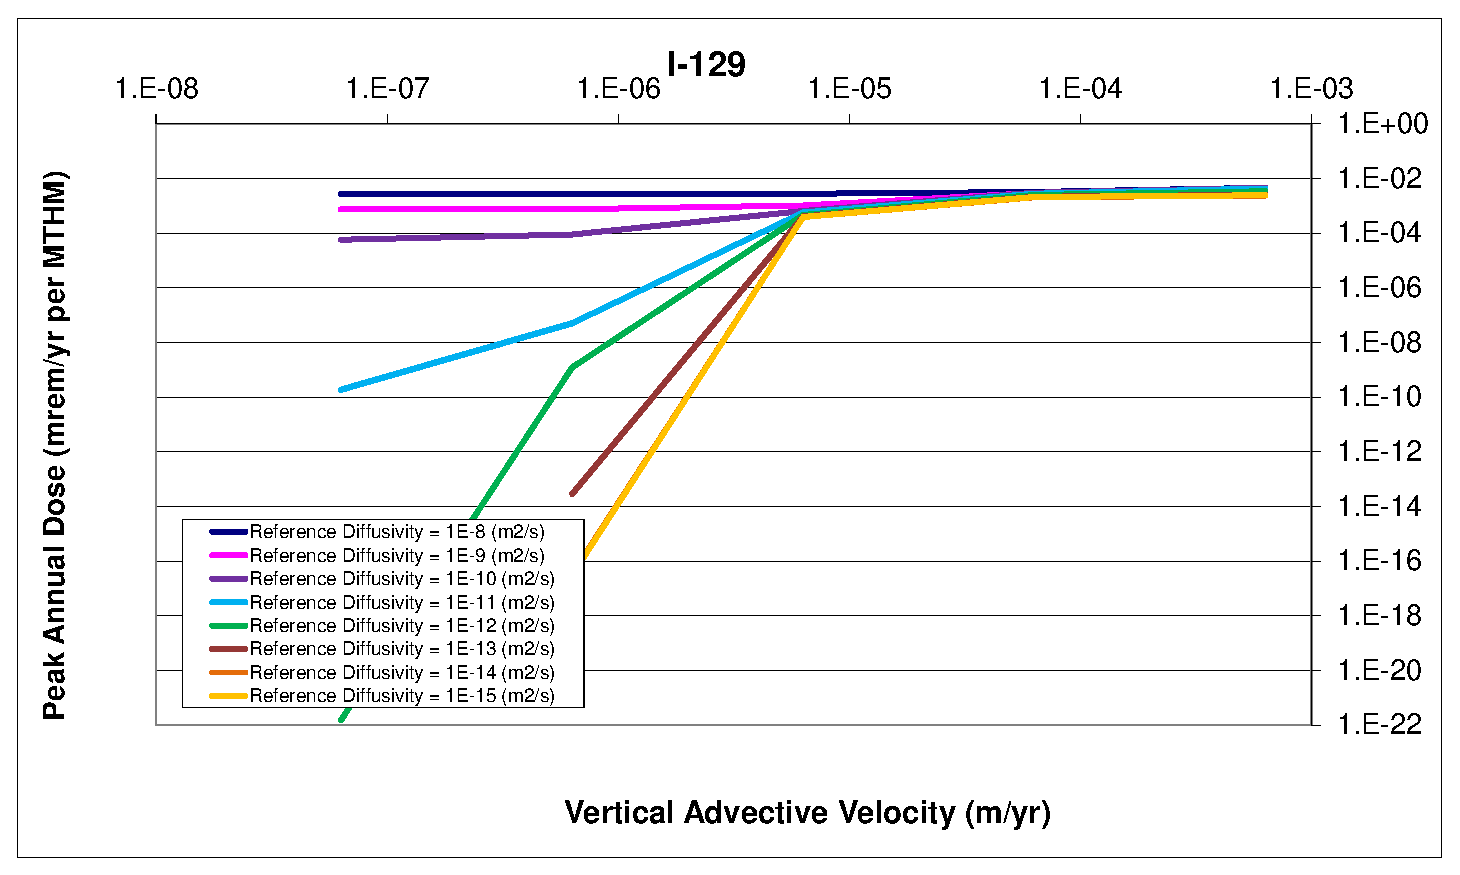
\includegraphics[width=\linewidth]{./chapters/nuclide_sensitivity/clay/AdvVelAndDiffCoeffEBSFail/I-129-VAdvVel.eps}
\caption{$^{129}I$ vertical advective velocity sensitivity.}
\label{fig:VAdvVelI129VAdvVel}

\end{minipage}
\end{figure}

\begin{figure}[htp!]
\begin{minipage}[b]{0.45\linewidth}

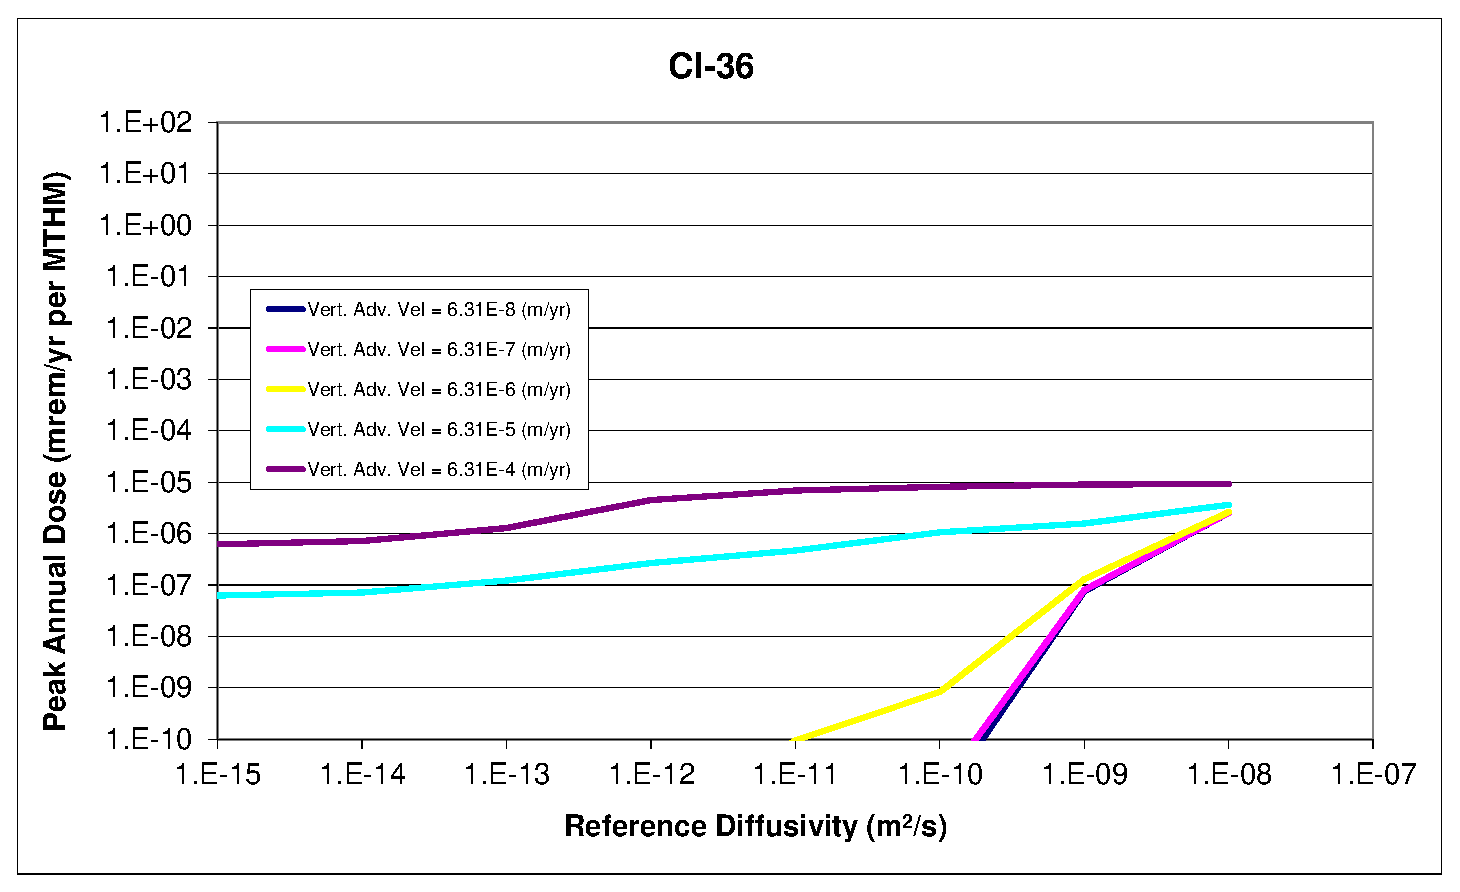
\includegraphics[width=\textwidth]{./chapters/nuclide_sensitivity/clay/AdvVelAndDiffCoeffEBSFail/Cl-36.eps}
\caption{$^{36}Cl$ reference diffusivity sensitivity.}
\label{fig:VAdvVelCl36}

\end{minipage}
\hspace{0.05\linewidth}
\begin{minipage}[b]{0.45\linewidth}

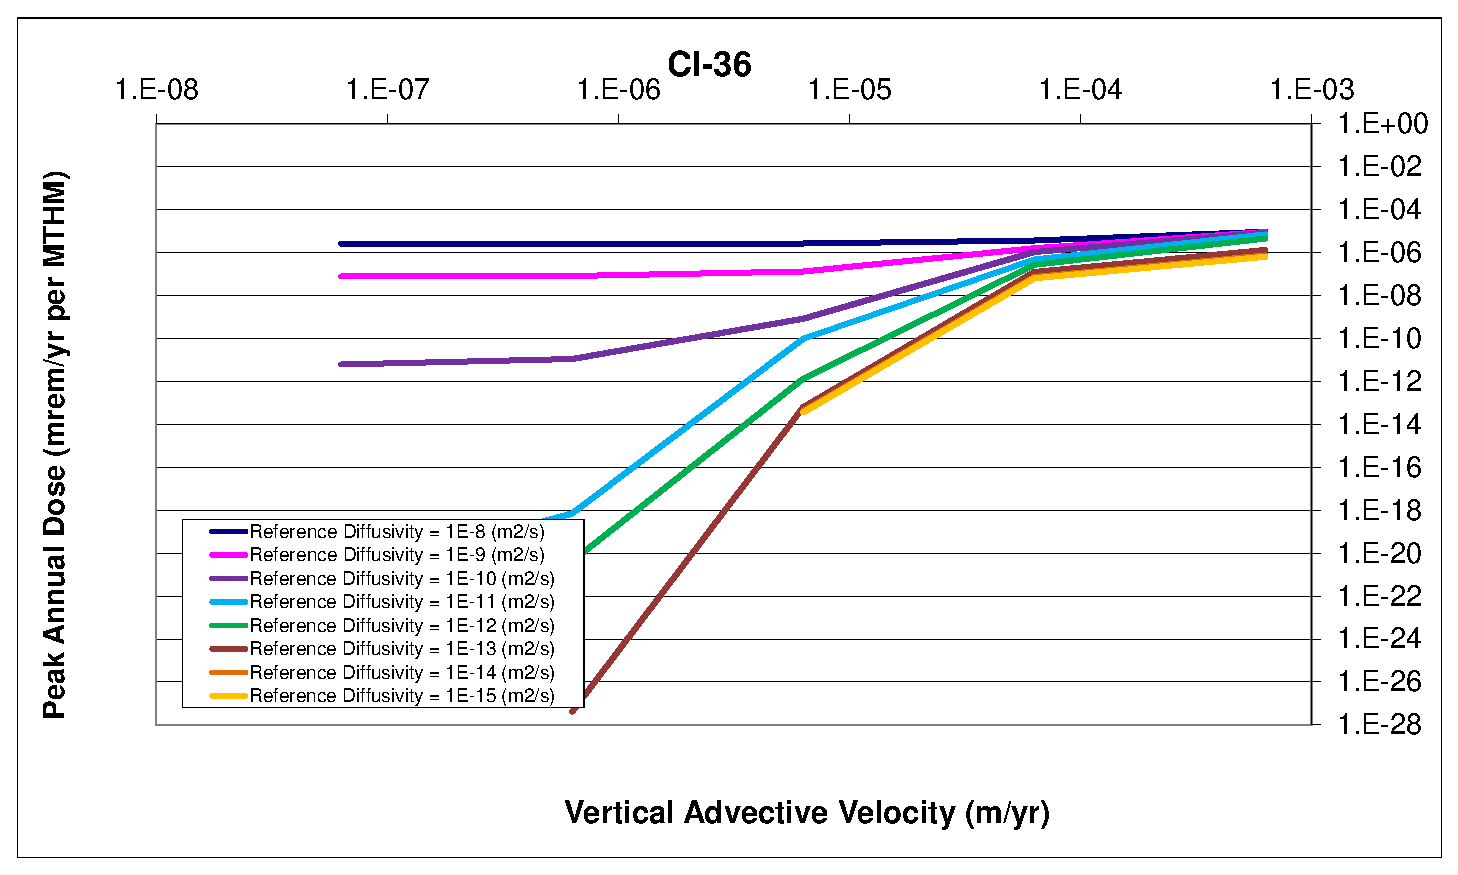
\includegraphics[width=\textwidth]{./chapters/nuclide_sensitivity/clay/AdvVelAndDiffCoeffEBSFail/Cl-36-VAdvVel.eps}
\caption{$^{36}Cl$ vertical advective velocity sensitivity.}
\label{fig:VAdvVelCl36VAdvVel}
\end{minipage}
\end{figure}

The solubility limited and sorbing elements, $Tc$ and $Np$, in Figures 
\ref{fig:VAdvVelTc99}, \ref{fig:VAdvVelTc99VAdvVel}, \ref{fig:VAdvVelNp237}, and 
\ref{fig:VAdvVelNp237VAdvVel} show a very weak influence on peak annual dose 
rate for low reference diffusivities, but show a direct proportionality between 
dose and reference diffusivity above a threshold. For $^{99}Tc$, for example, 
that threshold occurs at $1\times10^{-11}$ m$^2$/s. 


Dose contribution from $^{99}Tc$ has a proportional 
relationship with vertical advective velocity above a regime threshold at 
$6.31\times10^{-5}$ m/yr, above which the system exhibits sensitivity to 
advection. 

%There is an interesting feature in which $^{99}Tc$ 
%exhibits a decrease in peak annual dose for an increase in reference diffusivity 
%for the very high ($6.31\times10^{-4}$) vertcial advective velocity case. %WHY? 

\begin{figure}[htp!]
\begin{minipage}[b]{0.45\linewidth}
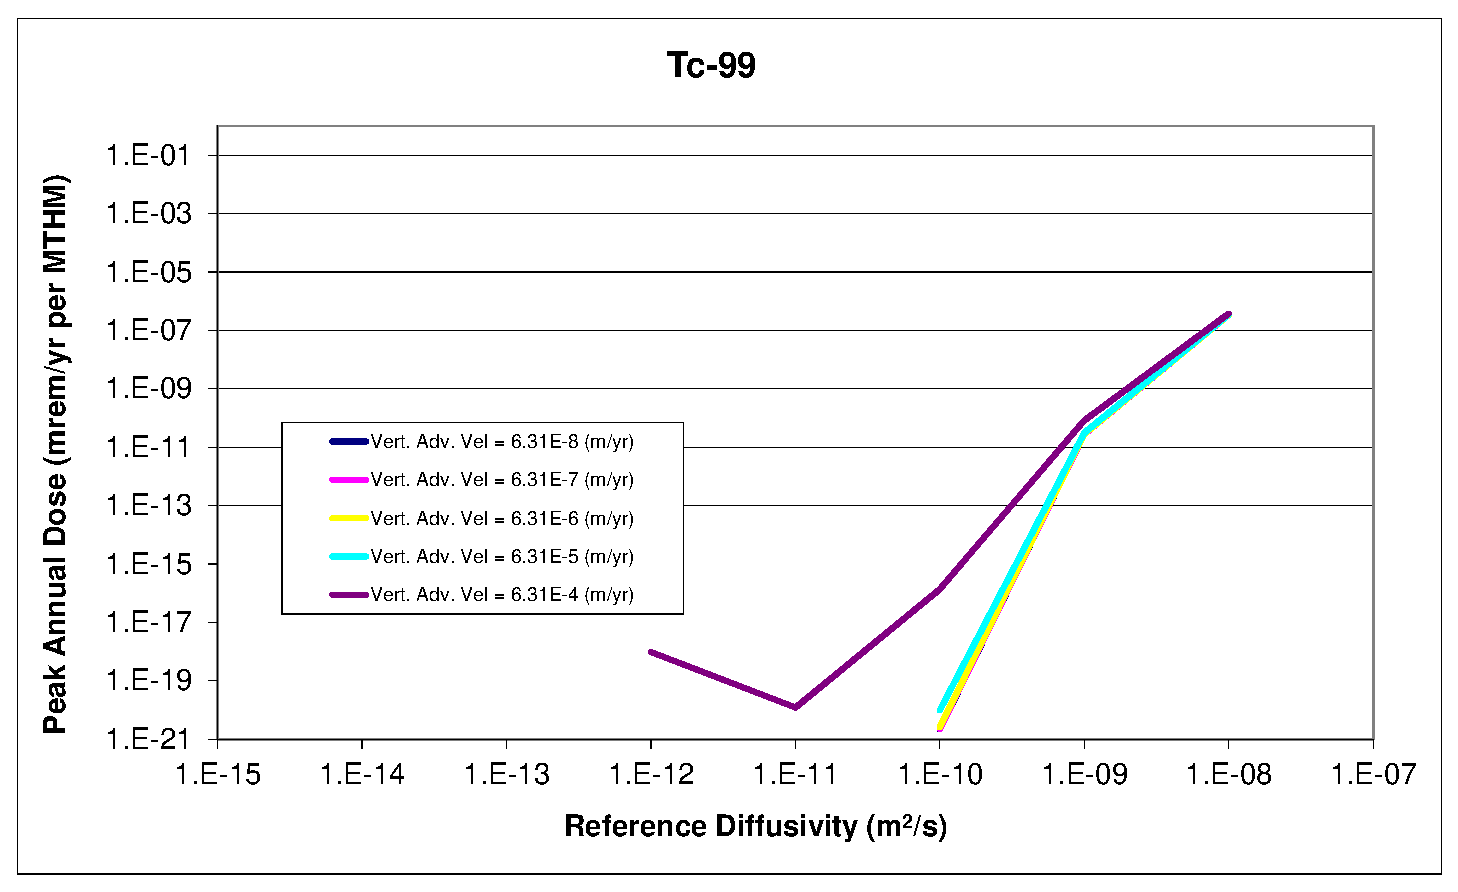
\includegraphics[width=\linewidth]{./chapters/nuclide_sensitivity/clay/AdvVelAndDiffCoeffEBSFail/Tc-99.eps}
\caption{$^{99}Tc$ reference diffusivity sensitivity.}
\label{fig:VAdvVelTc99}

\end{minipage}
\hspace{0.05\linewidth}
\begin{minipage}[b]{0.45\linewidth}

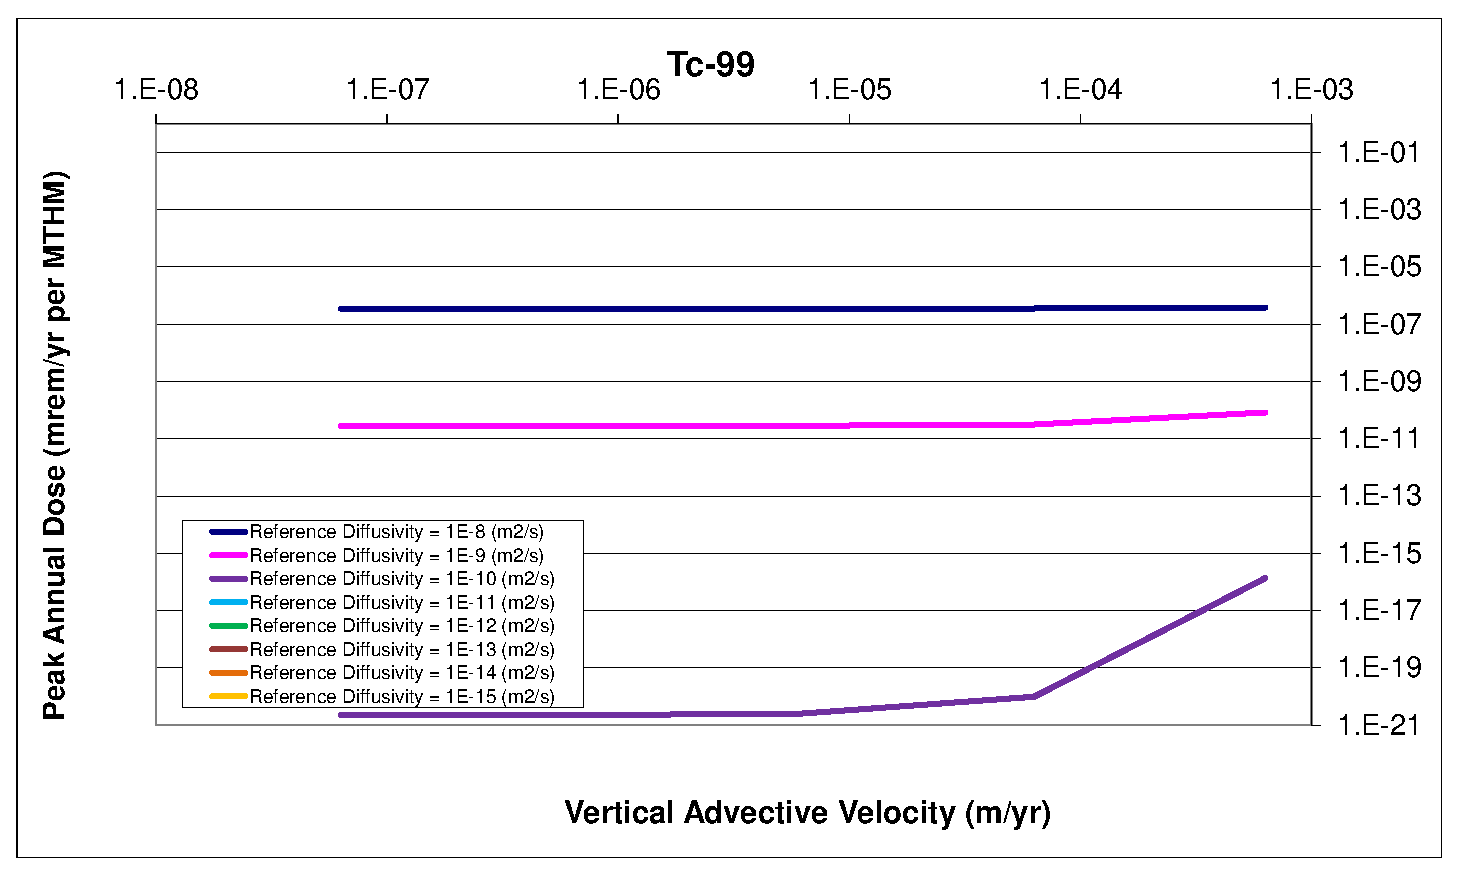
\includegraphics[width=\linewidth]{./chapters/nuclide_sensitivity/clay/AdvVelAndDiffCoeffEBSFail/Tc-99-VAdvVel.eps}
\caption{$^{99}Tc$ vertical advective velocity sensitivity.}
\label{fig:VAdvVelTc99VAdvVel}

\end{minipage}
\end{figure}

\begin{figure}[htp!]
\begin{minipage}[b]{0.45\linewidth}
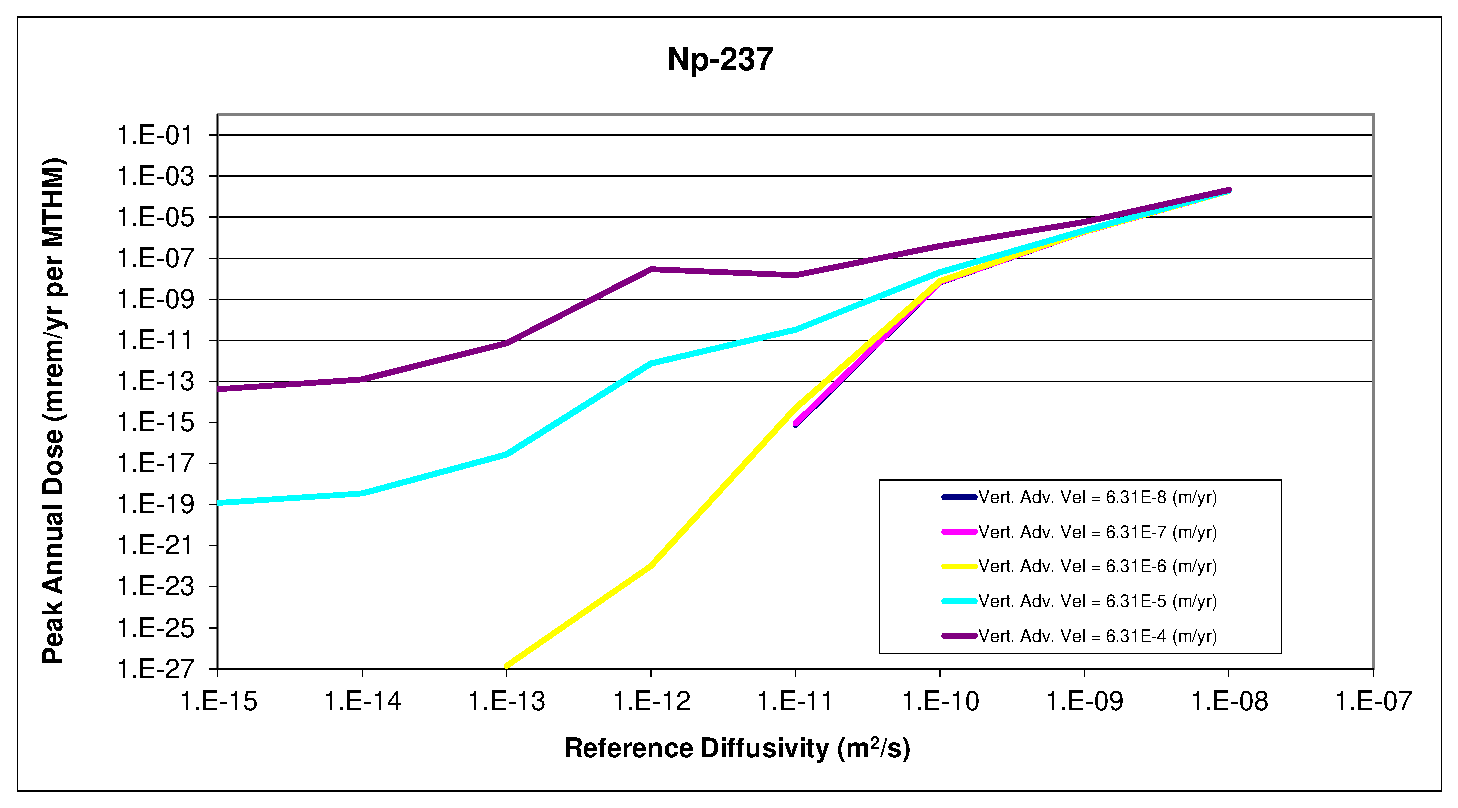
\includegraphics[width=\linewidth]{./chapters/nuclide_sensitivity/clay/AdvVelAndDiffCoeffEBSFail/Np-237.eps}
\caption{$^{237}Np$ reference diffusivity sensitivity.}
\label{fig:VAdvVelNp237}

\end{minipage}
\hspace{0.05\linewidth}
\begin{minipage}[b]{0.45\linewidth}

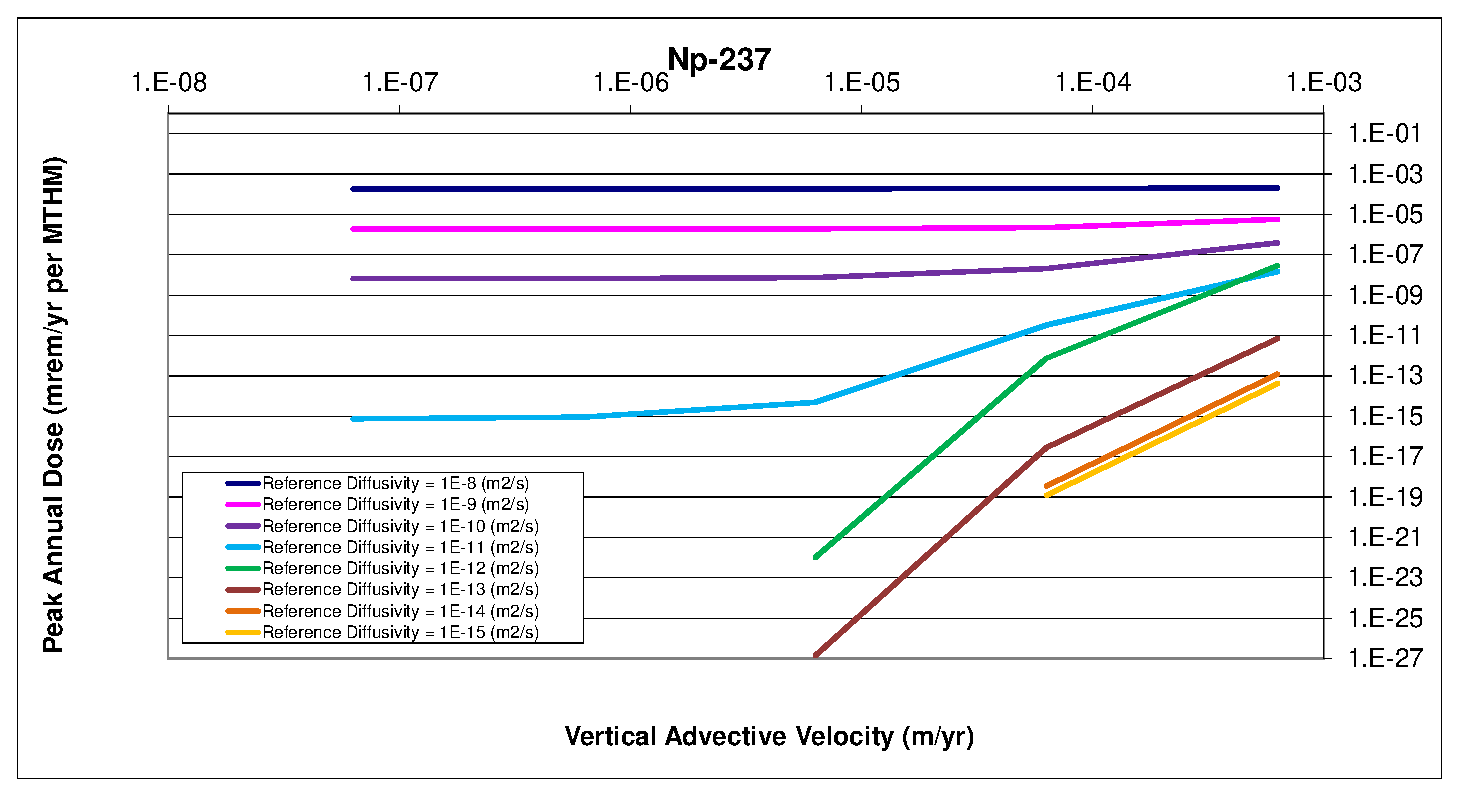
\includegraphics[width=\linewidth]{./chapters/nuclide_sensitivity/clay/AdvVelAndDiffCoeffEBSFail/Np-237-VAdvVel.eps}
\caption{$^{237}Np$ vertical advective velocity sensitivity.}
\label{fig:VAdvVelNp237VAdvVel}
  
\end{minipage}
\end{figure}

The convergence of the effect of the reference diffusivity and vertical 
advective velocity for the cases above shows the effect of dissolved 
concentration (solubility) limits and sorption. $Se$ is non-sorbing, but 
solubility limited.  The results from $^{79}Se$ in Figure \ref{fig:VAdvVelSe79} 
and \ref{fig:VAdvVelSe79VAdvVel} show that for low vertical advective velocity, 
the system is diffusion dominated.  However, for high vertical advective 
velocity, the diffusivity remains important even in the advective regime as 
spreading facilitates transport in the presence of solubility limited transport. 

\begin{figure}[htp!]
\begin{minipage}[b]{0.45\linewidth}
\centering
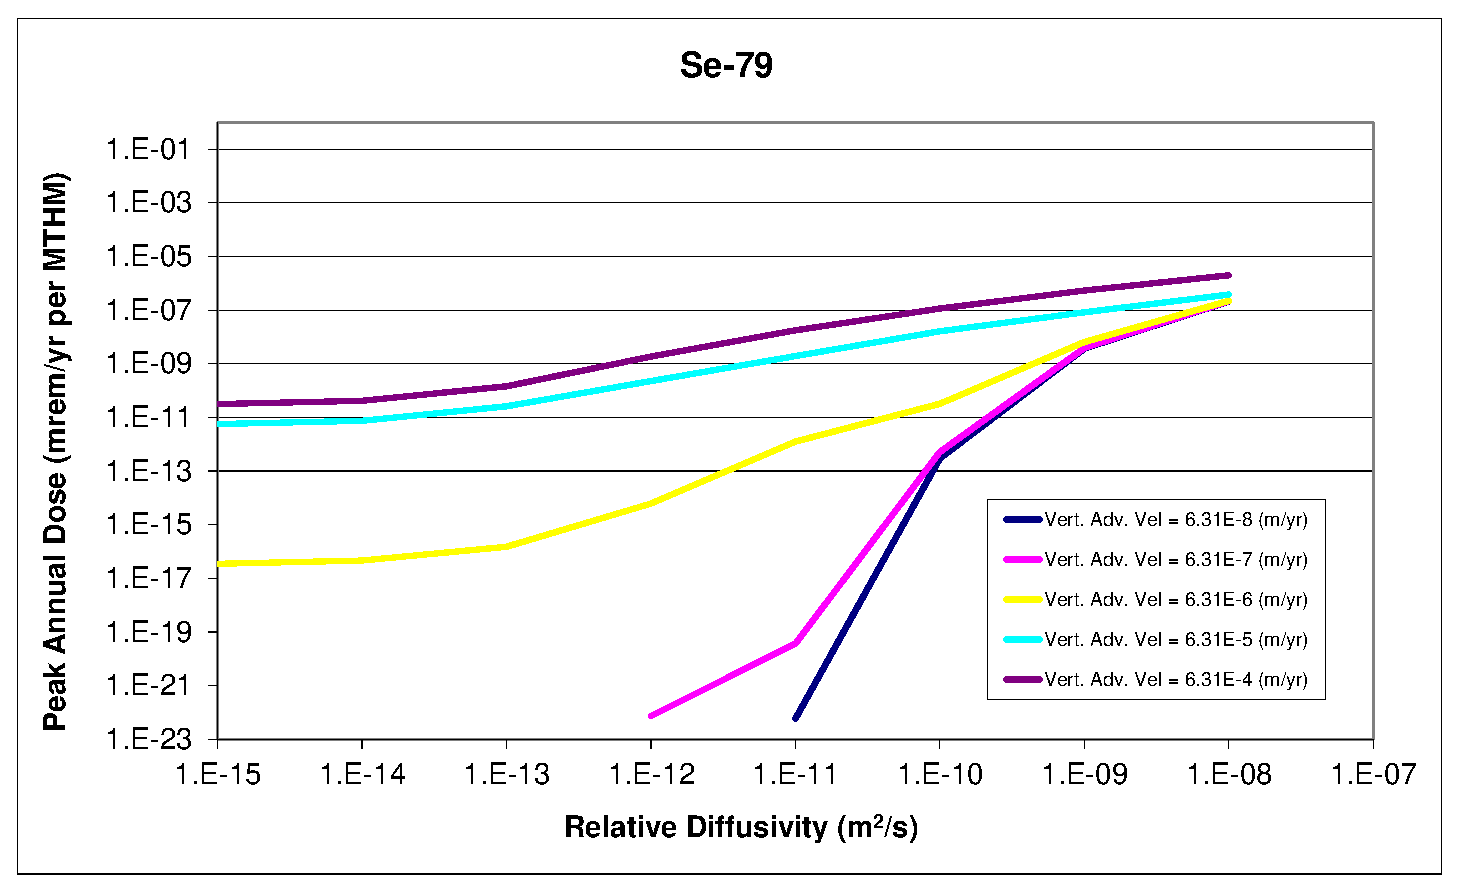
\includegraphics[width=\linewidth]{./chapters/nuclide_sensitivity/clay/AdvVelAndDiffCoeffEBSFail/Se-79.eps}
\caption{$^{79}Se$ reference diffusivity sensitivity.}
\label{fig:VAdvVelSe79}

\end{minipage}
\hspace{0.05\linewidth}
\begin{minipage}[b]{0.45\linewidth}

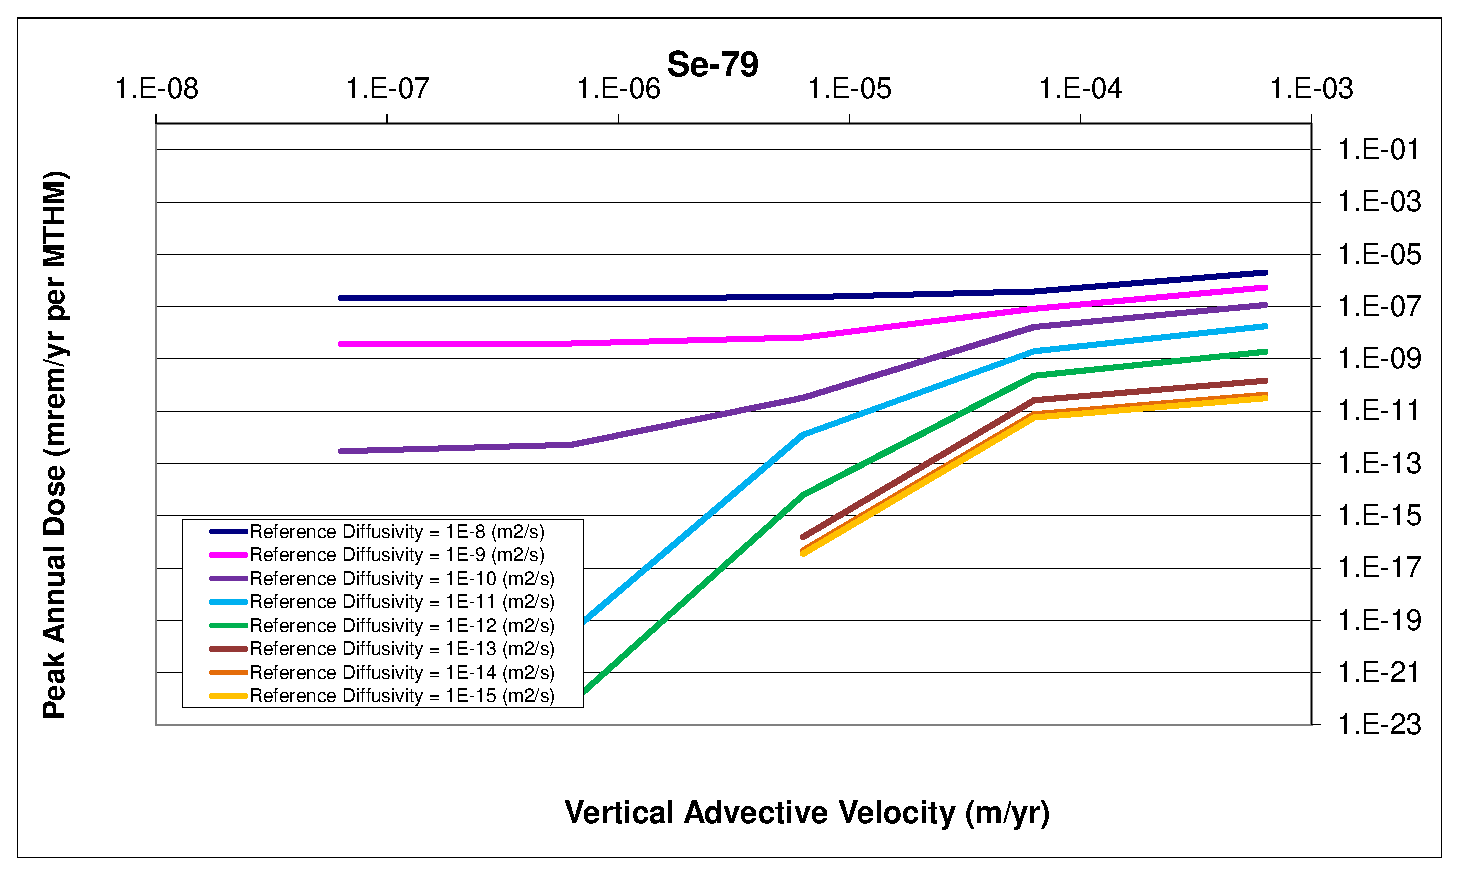
\includegraphics[width=\linewidth]{./chapters/nuclide_sensitivity/clay/AdvVelAndDiffCoeffEBSFail/Se-79-VAdvVel.eps}
\caption{$^{79}Se$ vertical advective velocity sensitivity.}
\label{fig:VAdvVelSe79VAdvVel}

\end{minipage}
\end{figure}
\FloatBarrier

\begin{frame}[ctb!]
\frametitle{Cyder Advective Diffusive Sensitivity}
\begin{figure}[ht]
\centering
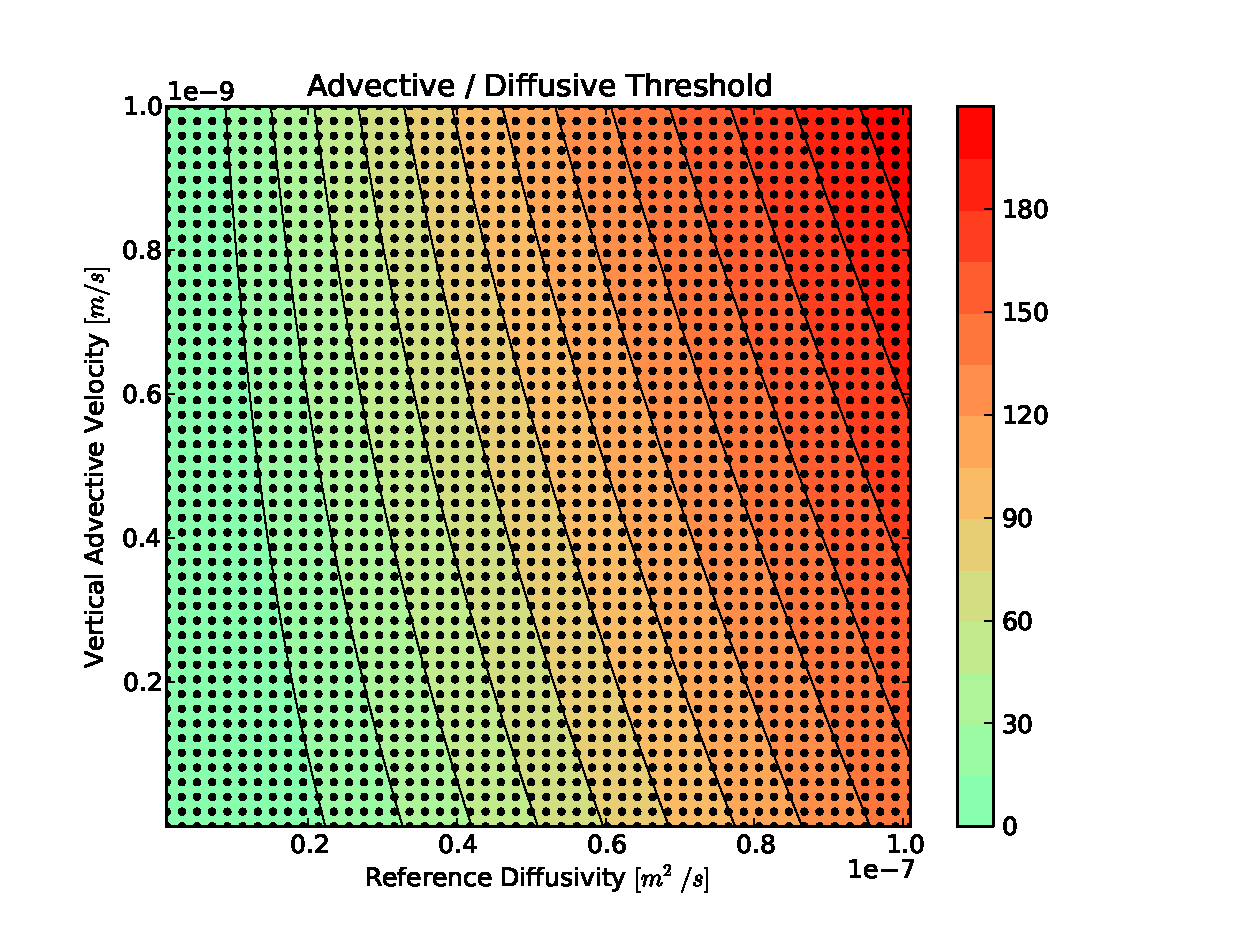
\includegraphics[height=0.7\textheight]{./nuclide_demonstration/adv_vel_diff.eps}
\caption[Advection vs. Diffusion Sensitivity in Cyder]{Dual advective velocity 
and reference diffusivity sensitivity for a non-sorbing, infinitely soluble 
nuclide. This demonstration utilized the Degradation Rate model and the coupled 
advective dispersive mass transfer mode.}
\label{fig:dr_adv_diff}
\end{figure}
\end{frame}


\FloatBarrier
\subsection{Case II : Solubility Sensitivity}
\begin{frame}[ctb!]
\frametitle{Clay GDSM Solubility Sensitivity}
\begin{figure}[htb!]
\centering
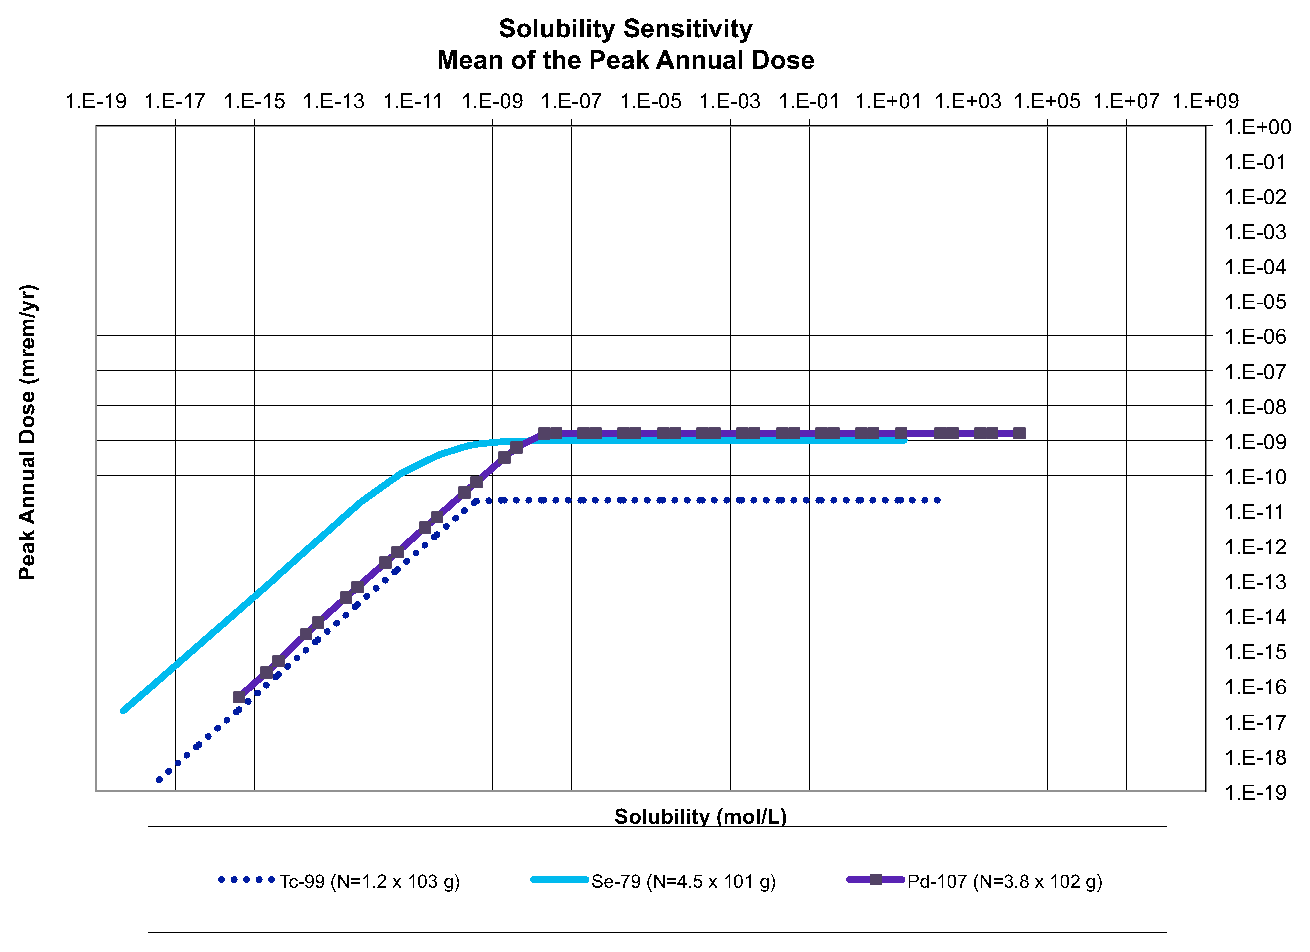
\includegraphics[width=0.7\linewidth]{./nuclide_demonstration/Solubility_Summary_Sol.eps}
\caption{Solubility limit sensitivity. The peak annual dose due to an inventory, 
$N$, of each isotope.}
\label{fig:SolSum}
\end{figure}
\end{frame}


\FloatBarrier
\subsection{Case III : Sorption Sensitivity}


\subsubsection{Reference Sorption Coefficient Sensitivity}

In the parametric sensitivity analysis discussed in Section \ref{sec:sorption}, 
the expected inverse relationship between the retardation factor and resulting 
peak annual dose was found for all elements that were not assumed to be 
effectively infinitely soluble. In the low retardation coefficient cases, a 
regime is established in which the peak annual dose is entirely unaffected by 
changes in retardation coefficient. For large values of retardation 
coefficient, the sensitivity to small changes in the retardation coefficient 
increases dramatically. In that sensitive regime, the change in peak annual 
dose is inversely related to the retardation coefficient. Between these two 
regimes was a transition regime, in which the $K_d$ factor ranges from 
$1\times10^{-5}$ to $5\times10^{0} [-]$.

It is clear from Figures \ref{fig:KdSumFactor} and \ref{fig:KdSum} that 
for retardation coefficients greater than a threshold, the 
relationship between peak annual dose and retardation coefficient is a strong 
inverse one. 

\begin{figure}[ht]
\centering
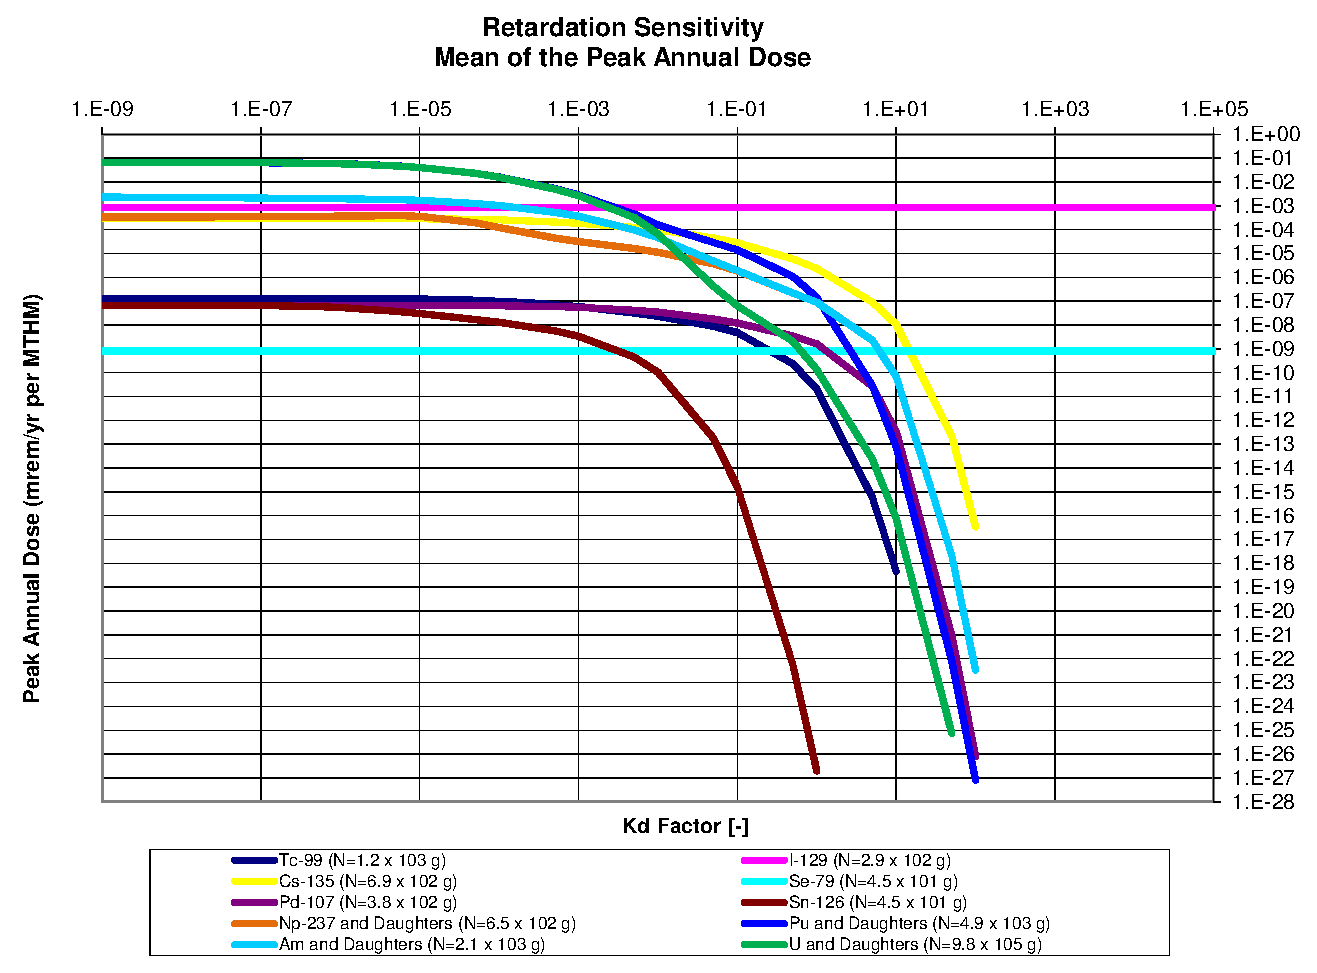
\includegraphics[width=0.7\linewidth]{./chapters/nuclide_sensitivity/clay/Sorption/Retardation_Summary_kdFactor.eps}
\caption{$K_d$ factor sensitivity.  The peak annual dose due to an inventory, 
$N$, of each isotope.}
\label{fig:KdSumFactor}
\end{figure}

\begin{figure}[ht]
\centering
\includegraphics[width=0.7\linewidth]{./chapters/nuclide_sensitivity/clay/Sorption/Retardation_Summary_kd.eps}
\caption{$K_d$ sensitivity.  The peak annual dose due to an inventory, 
$N$, of each isotope.}
\label{fig:KdSum}
\end{figure}

\clearpage


\subsubsection{Reference Sorption Coefficient Sensitivity}

In the parametric analysis of \Cyder performance, it was shown that sorption 
sensitivity behavior closely matched that of the \gls{GDSM} sensitivity 
behaviors. Specifically, in Figure \ref{fig:kd_result}, increasing the retardation 
coefficient results in a smooth but dramatic turnover. 

\begin{figure}[ht]
\centering
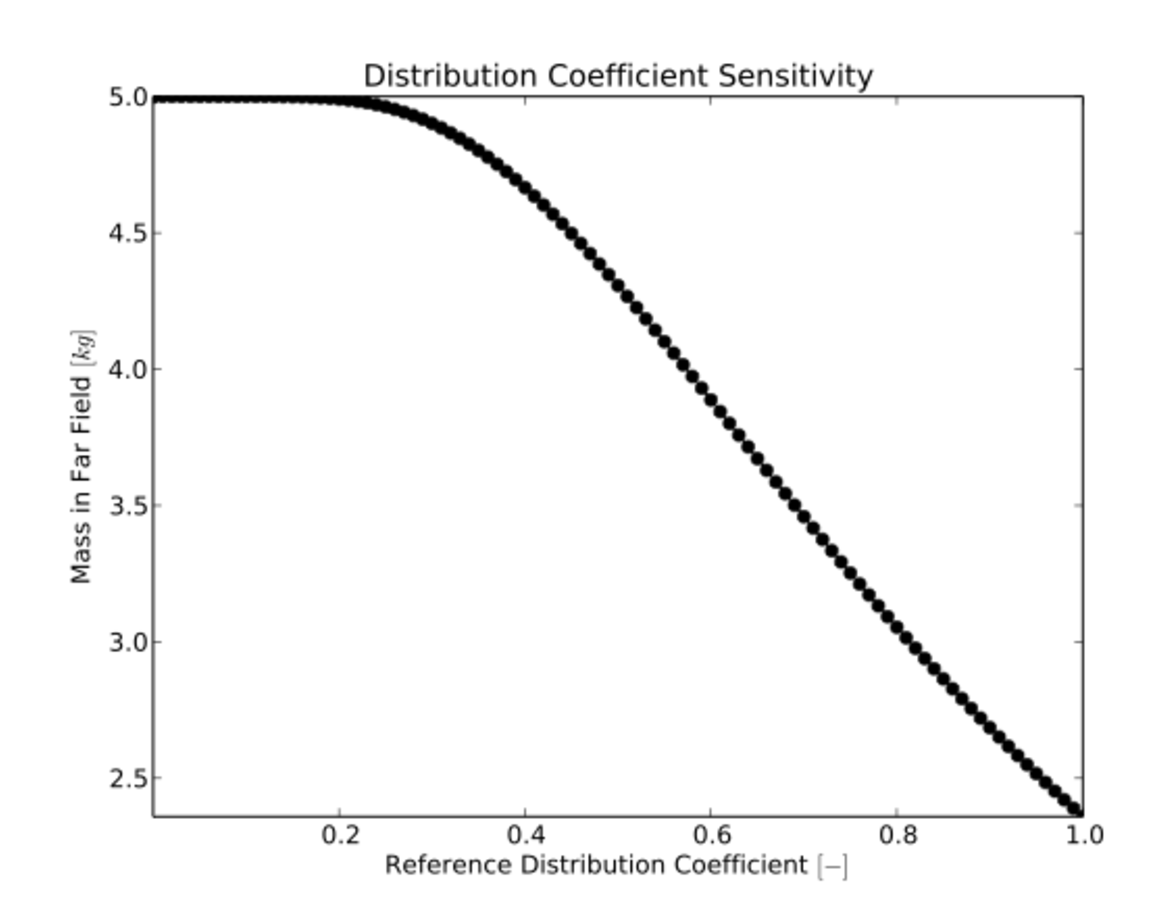
\includegraphics[width=0.7\linewidth]{./chapters/demonstration/bench/kd.eps}
\caption[$K_d$ sensitivity in the Mixed Cell Model]{$K_d$ sensitivity in the 
\Cyder tool for an arbitrary isotope assigned a variable $K_d$ coefficient.} 
\label{fig:kd_result}
\end{figure}


\FloatBarrier
\subsection{Case IV : Waste Form Degradation Rate and Inventory Sensitivity}
\subsubsection{Waste Form Degradation Rate and Contaminant Inventory Sensitivity}

In the parametric sensitivity analysis discussed in Section 
\ref{sec:wfdeginv}, the results showed two regimes. In the first regime, 
the mean of the peak annual dose rates is directly proportional to both the mass 
factor and the fractional waste form degradation rate. For some radionuclides, 
attenuation occurs for high values of both parameters as the release of 
radionuclides is limited by dispersion parameters. This phenomenon can be seen 
in the figures below in which transition between regimes for higher degradation 
rates happens at lower mass factors than transition between regimes for lower 
degradation rates. 

The peaks for highly soluble, non sorbing elements such as $I$ and $Cl$
are directly proportional to mass factor for most 
values of waste form degradation rates. This effect can be seen in Figures 
\ref{fig:WFDegI129}, \ref{fig:WFDegI129MF}, \ref{fig:WFDegCl36}, and 
\ref{fig:WFDegCl36MF}. 


Highly soluble and non-sorbing $^{129}I$ demonstrates a direct proportionality between dose rate and 
fractional degradation rate until a turnover where other natural system 
parameters dampen transport. Highly soluble and non-sorbing $^{129}I$ domonstrates a direct 
proportionality to the inventory multiplier.

\begin{figure}[ht!]
\begin{minipage}[b]{0.45\linewidth}
\centering
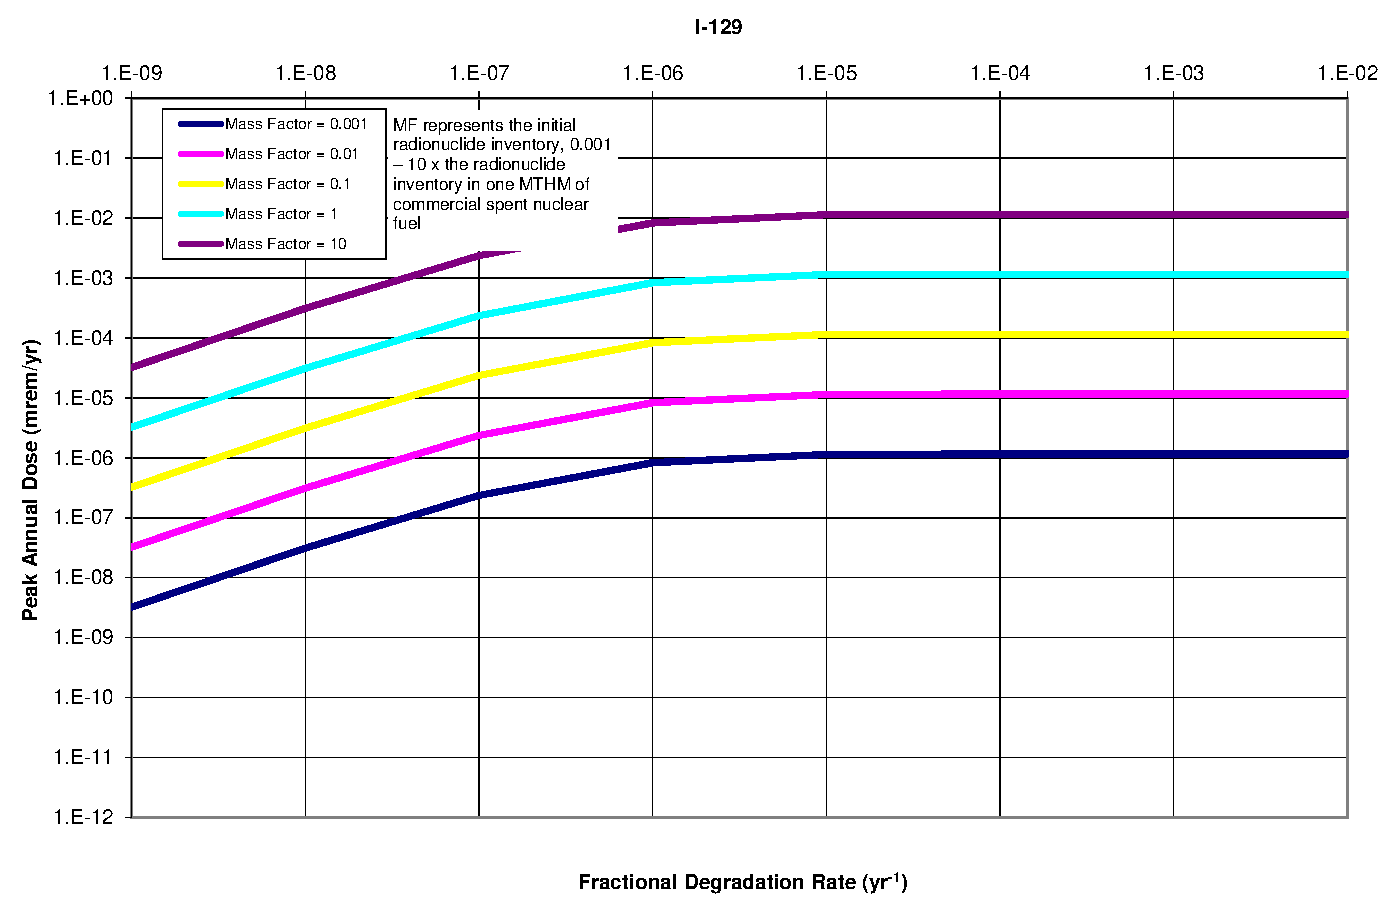
\includegraphics[width=\linewidth]{./chapters/nuclide_sensitivity/clay/WFDegAndInv/I-129.eps}
\caption{$^{129}I$ waste form degradation rate sensitivity.}
\label{fig:WFDegI129}

\end{minipage}
\hspace{0.05\linewidth}
\begin{minipage}[b]{0.45\linewidth}

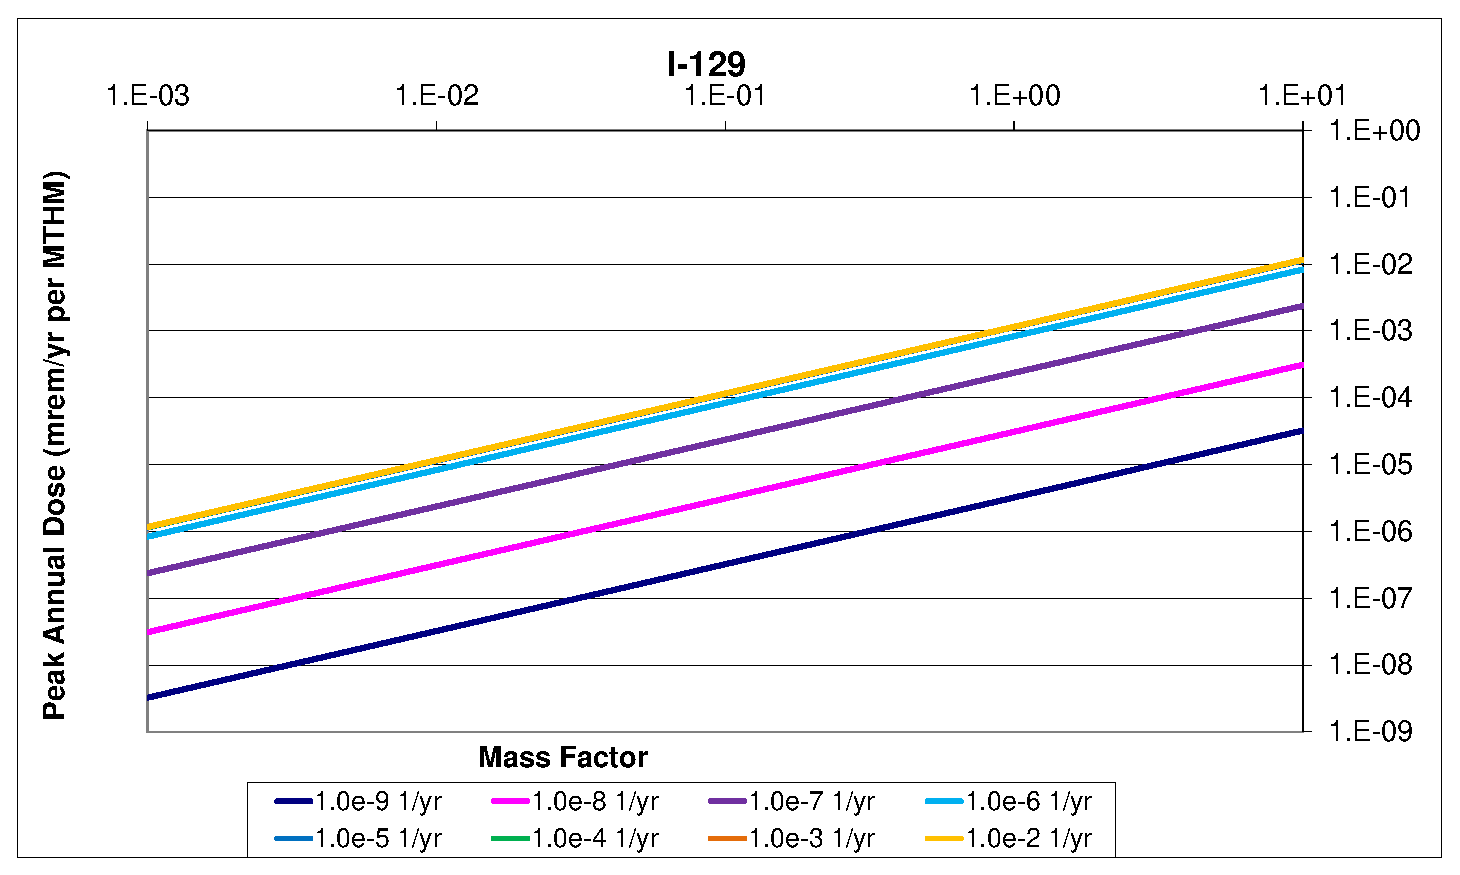
\includegraphics[width=\linewidth]{./chapters/nuclide_sensitivity/clay/WFDegAndInv/I-129-MF.eps}
\caption{$^{129}I$ inventory multiplier sensitivity.}
\label{fig:WFDegI129MF}

\end{minipage}
\end{figure}
\begin{figure}[ht]
\begin{minipage}[b]{0.45\linewidth}

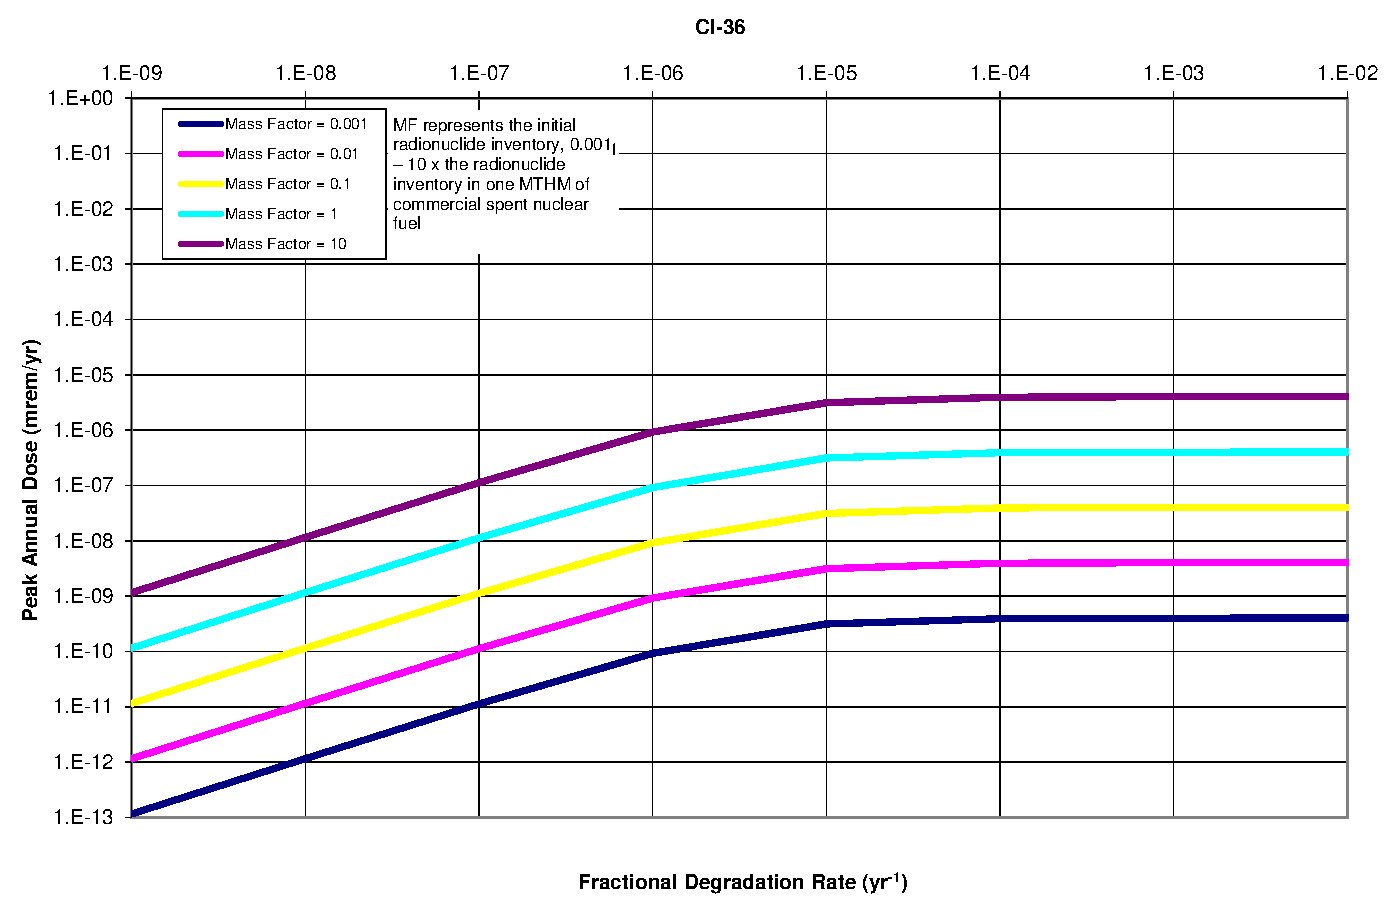
\includegraphics[width=\linewidth]{./chapters/nuclide_sensitivity/clay/WFDegAndInv/Cl-36.eps}
\caption{$^{36}Cl$ waste form degradation rate sensitivity.}
\label{fig:WFDegCl36}

\end{minipage}
\hspace{0.05\linewidth}
\begin{minipage}[b]{0.45\linewidth}

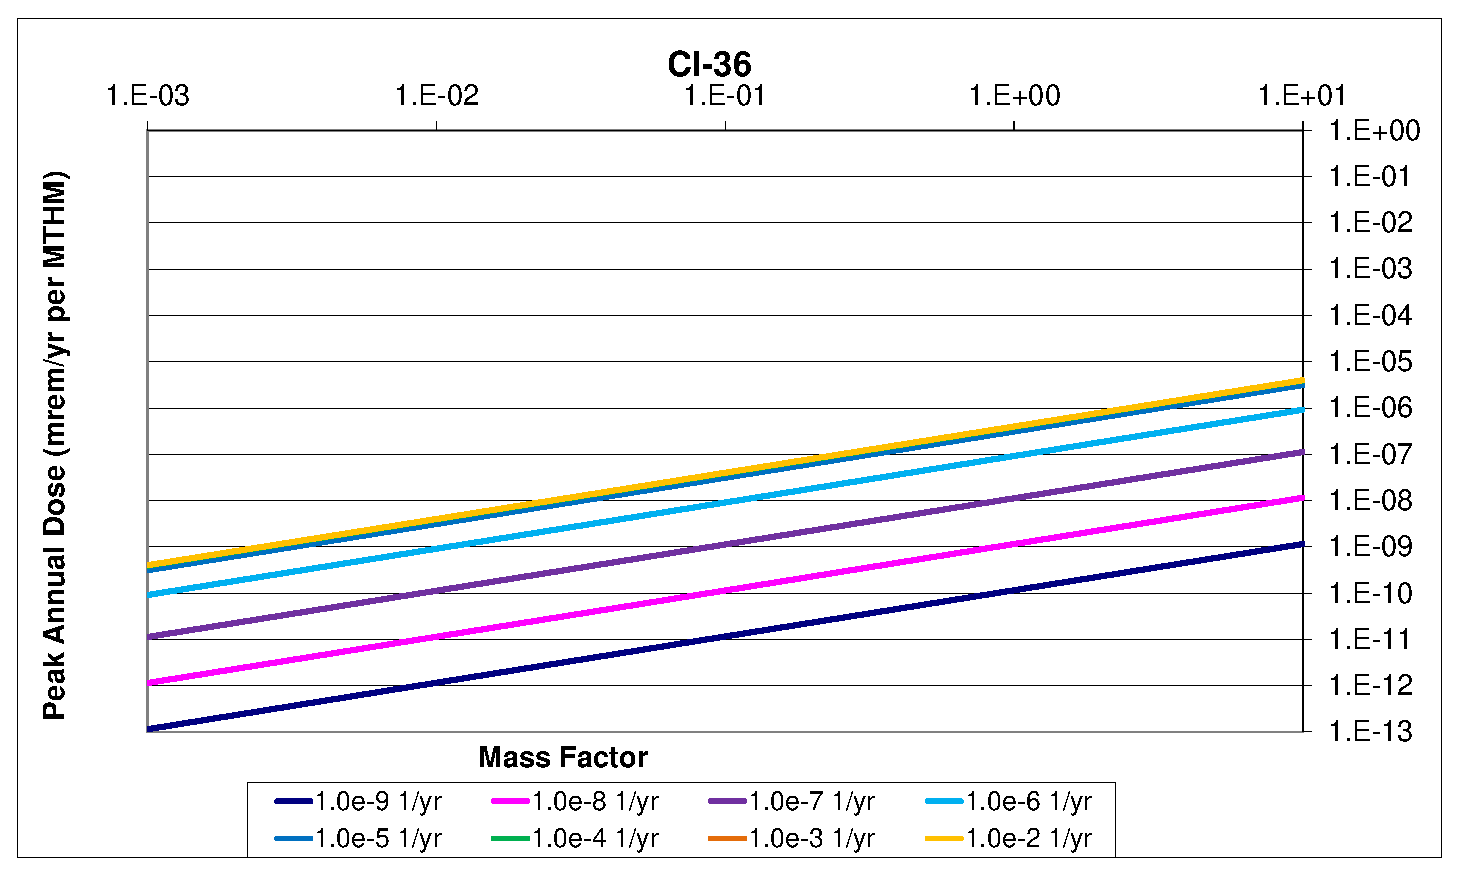
\includegraphics[width=\linewidth]{./chapters/nuclide_sensitivity/clay/WFDegAndInv/Cl-36-MF.eps}
\caption{$^{36}Cl$ inventory multiplier sensitivity.}
\label{fig:WFDegCl36MF}
\end{minipage}
\end{figure}

The peaks for solubility limited, sorbing elements such as $Tc$ and $Np$, on the 
other hand, have a more dramatic turnover.  For very high degradation rates, the 
dependence on mass factor starts to round off due to attenuation by solubility 
limits, as can be seen in Figures \ref{fig:WFDegNp237}, \ref{fig:WFDegNp237MF}, 
\ref{fig:WFDegTc99}, and \ref{fig:WFDegTc99MF}.

Solubility limited and sorbing $^{99}Tc$ demonstrates a direct proportionality 
to fractional degradation rate until attuation by its solubility limit and other 
natural system parameters.  

\begin{figure}[ht!]
\begin{minipage}[b]{0.45\linewidth}

\centering
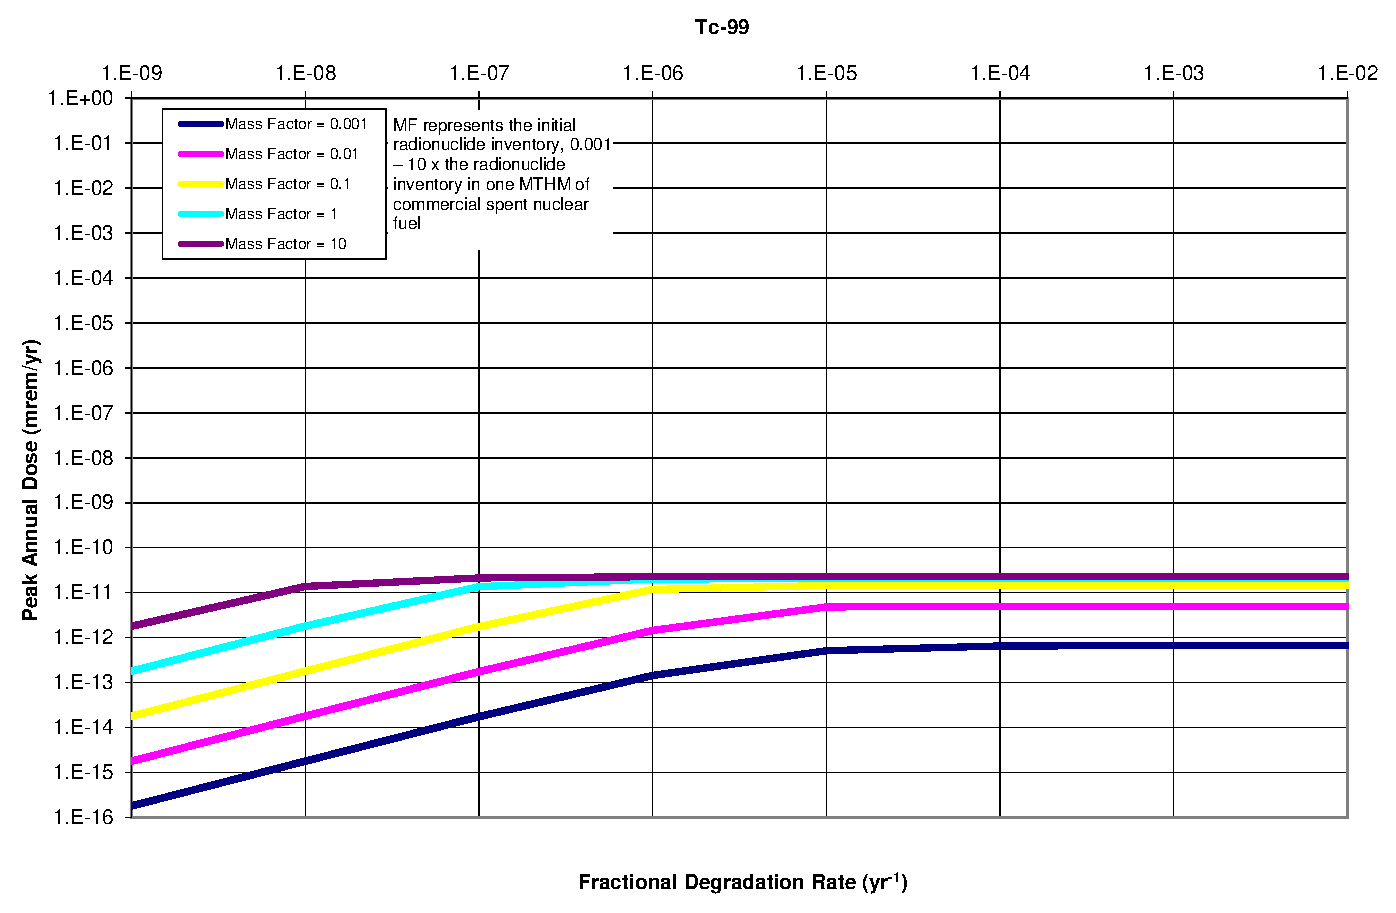
\includegraphics[width=\linewidth]{./chapters/nuclide_sensitivity/clay/WFDegAndInv/Tc-99.eps}
\caption{$^{99}Tc$ waste form degradation rate sensitivity.}
\label{fig:WFDegTc99}

\end{minipage}
\hspace{0.05\linewidth}
\begin{minipage}[b]{0.45\linewidth}

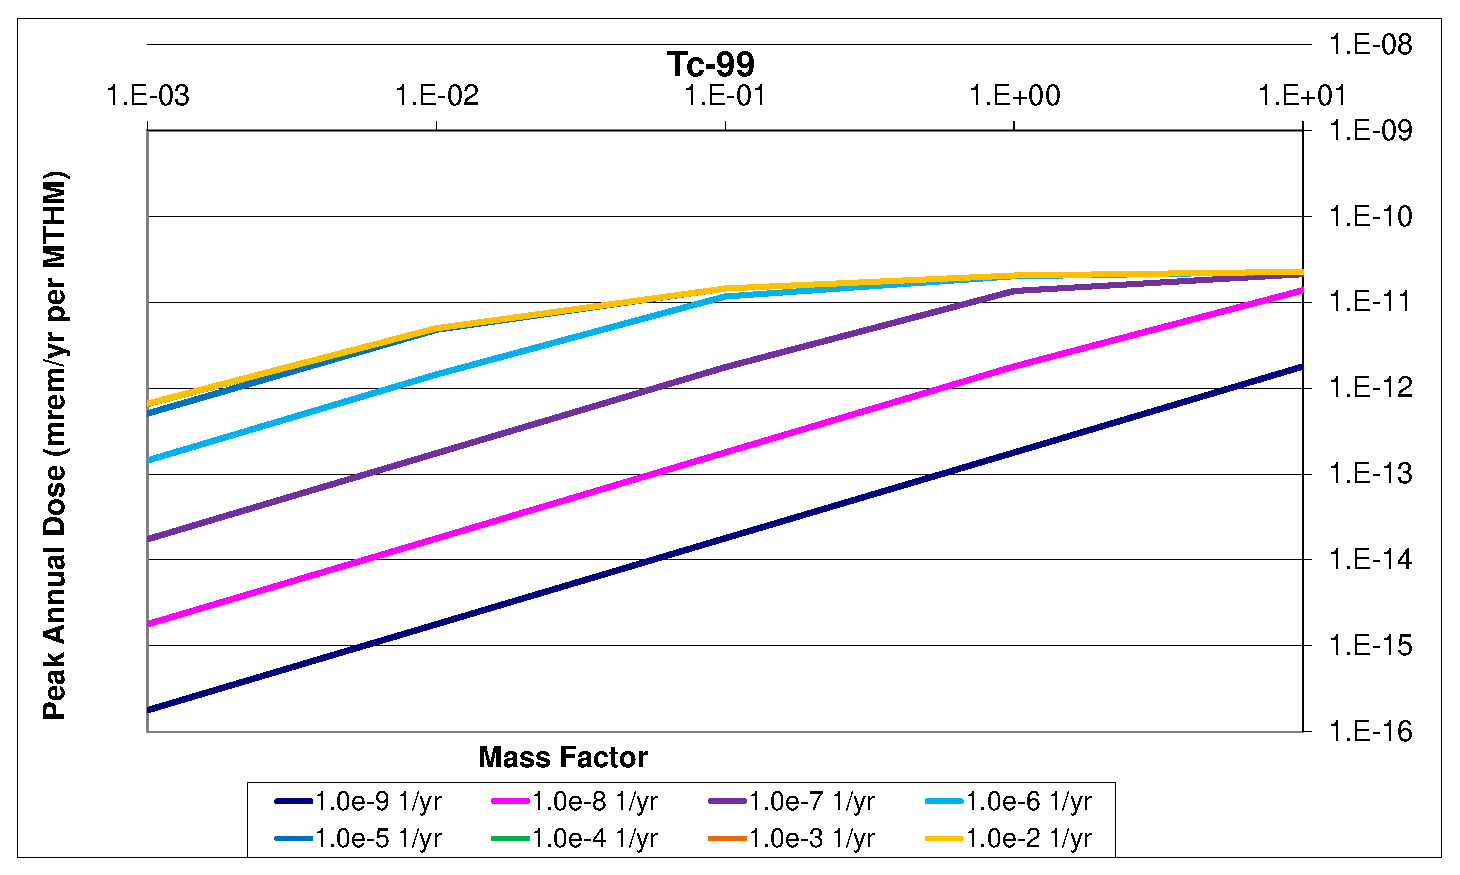
\includegraphics[width=\linewidth]{./chapters/nuclide_sensitivity/clay/WFDegAndInv/Tc-99-MF.eps}
\caption{$^{99}Tc$ inventory multiplier sensitivity.}
\label{fig:WFDegTc99MF}

\end{minipage}
\end{figure}
\begin{figure}[ht]
\begin{minipage}[b]{0.45\linewidth}

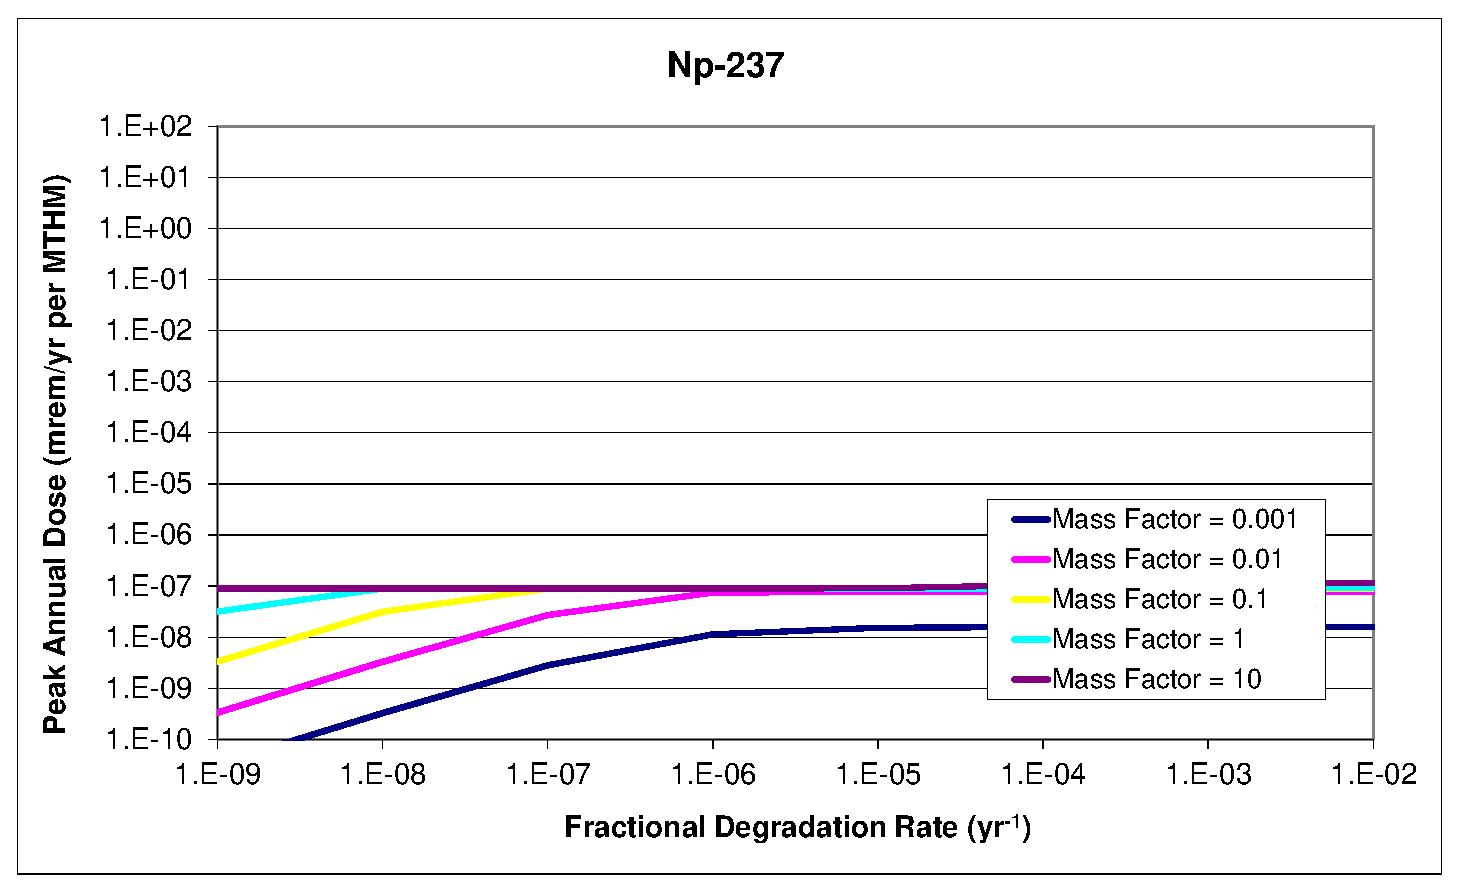
\includegraphics[width=\linewidth]{./chapters/nuclide_sensitivity/clay/WFDegAndInv/Np-237.eps}
\caption{$^{237}Np$ waste form degradation rate sensitivity.}
\label{fig:WFDegNp237}

\end{minipage}
\hspace{0.05\linewidth}
\begin{minipage}[b]{0.45\linewidth}

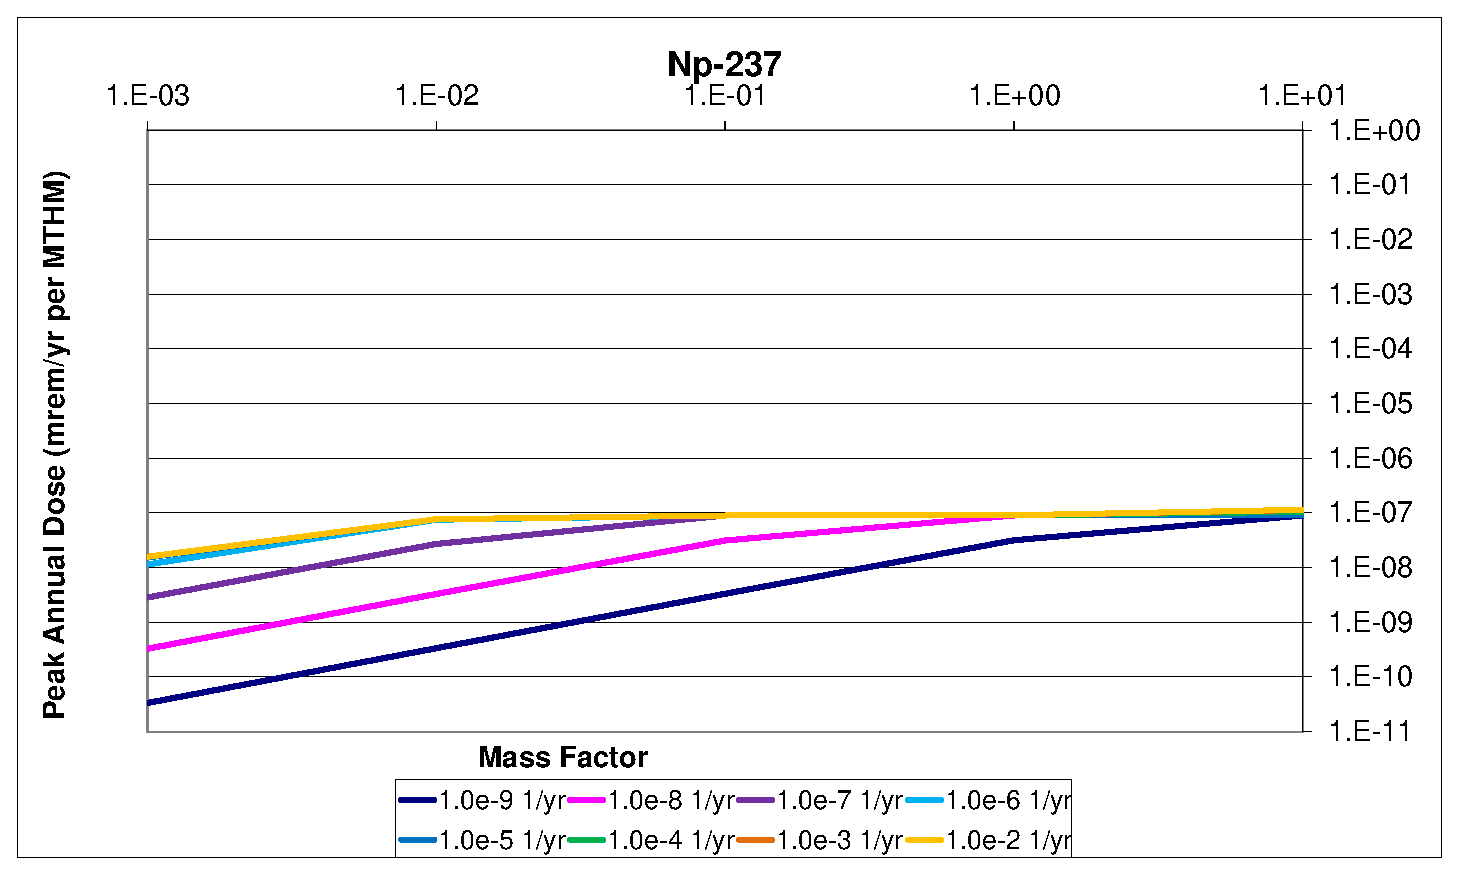
\includegraphics[width=\linewidth]{./chapters/nuclide_sensitivity/clay/WFDegAndInv/Np-237-MF.eps}
\caption{$^{237}Np$ inventory multiplier sensitivity.}
\label{fig:WFDegNp237MF}

\end{minipage}
\end{figure}
\FloatBarrier 


In the parametric sensitivity analysis conducted with the \Cyder tool, waste 
form degradation rate sensitvity similarly shows the two regimes noted in the 
\gls{GDSM} analysis.  


\begin{figure}[htbp!]
\begin{center}
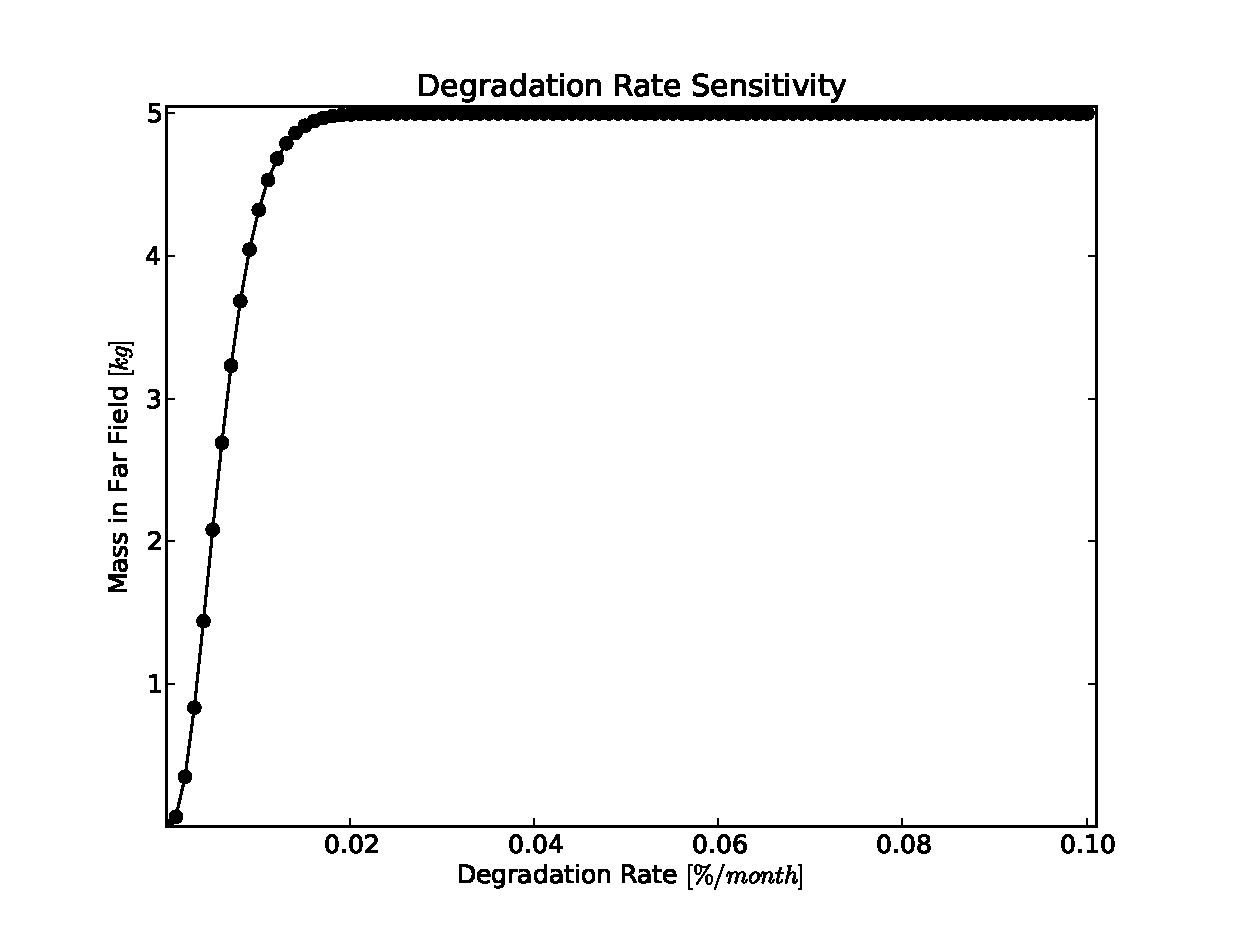
\includegraphics[width=0.7\linewidth]{./chapters/demonstration/bench/deg.eps}
\end{center}
\caption{Sensitivity demonstration of the degradation rate in \Cyder for an 
arbitrary isotope.}
\label{fig:deg}
\end{figure}


%\subsection{Case IVI : Waste Package Failure Time and Diffusion Coefficient Sensitivity}
%\subsubsection{Waste Package Failure Time Sensitivity}

In the parametric sensitivity analysis discussed in section 
\ref{sec:wpfail}, it was shown that For the clay repository, the waste 
package failure time is entirely irrelevant until waste package failure times 
reach the million or ten million year time scale. 

\begin{figure}[ht!]
  \centering
  \begin{minipage}[b]{0.45\linewidth}
    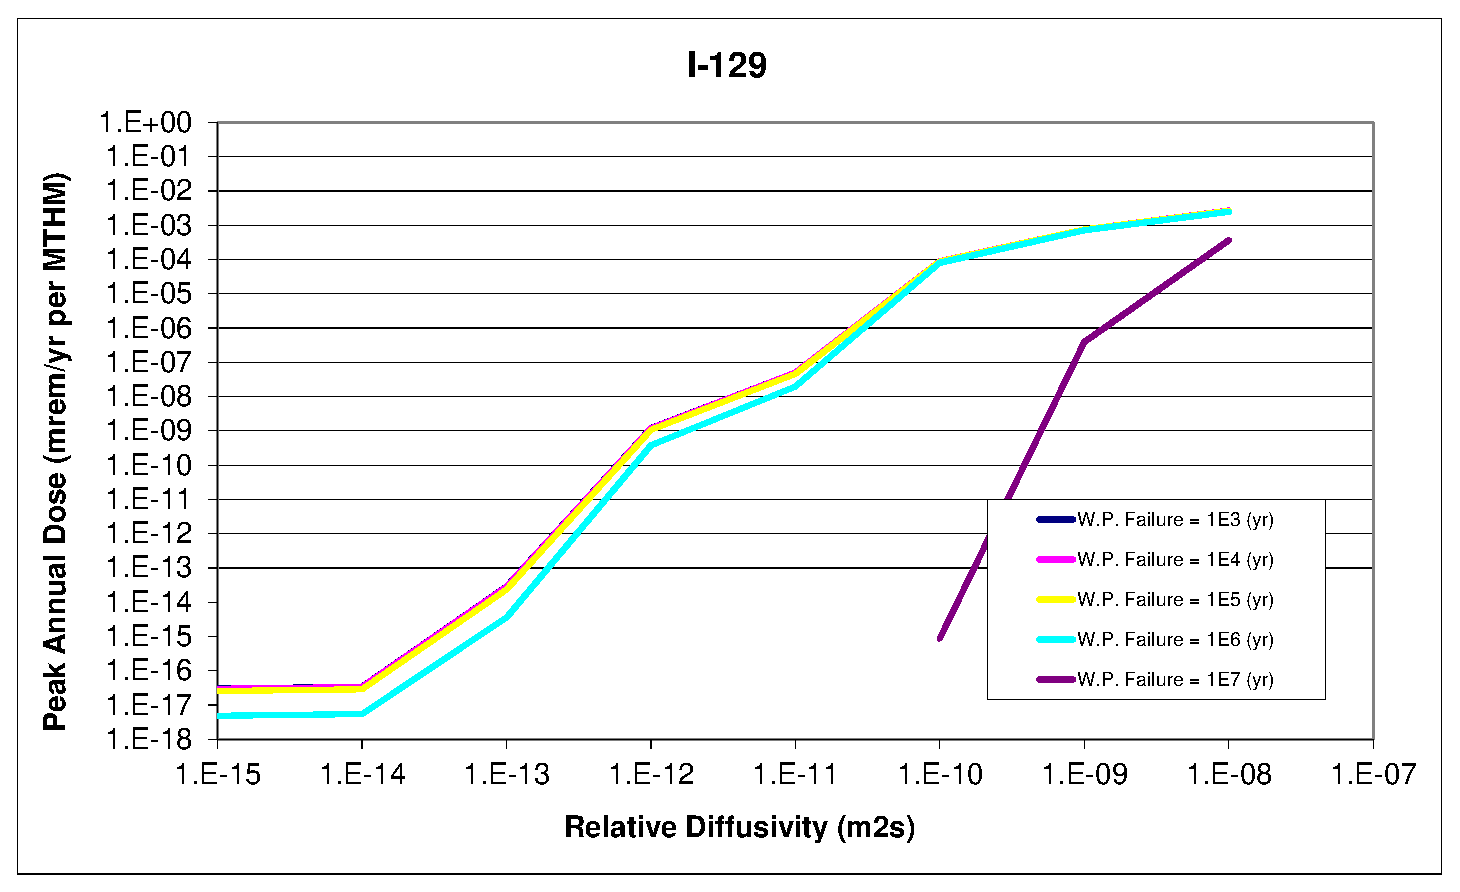
\includegraphics[width=\linewidth]{./chapters/nuclide_sensitivity/clay/WPFailExtended/I-129.eps}
    \caption{$^{129}I$ waste package failure time sensitivity. }
    \label{fig:WPFailI129}

  \end{minipage}
  \hspace{0.05\linewidth}
  \begin{minipage}[b]{0.45\linewidth}

    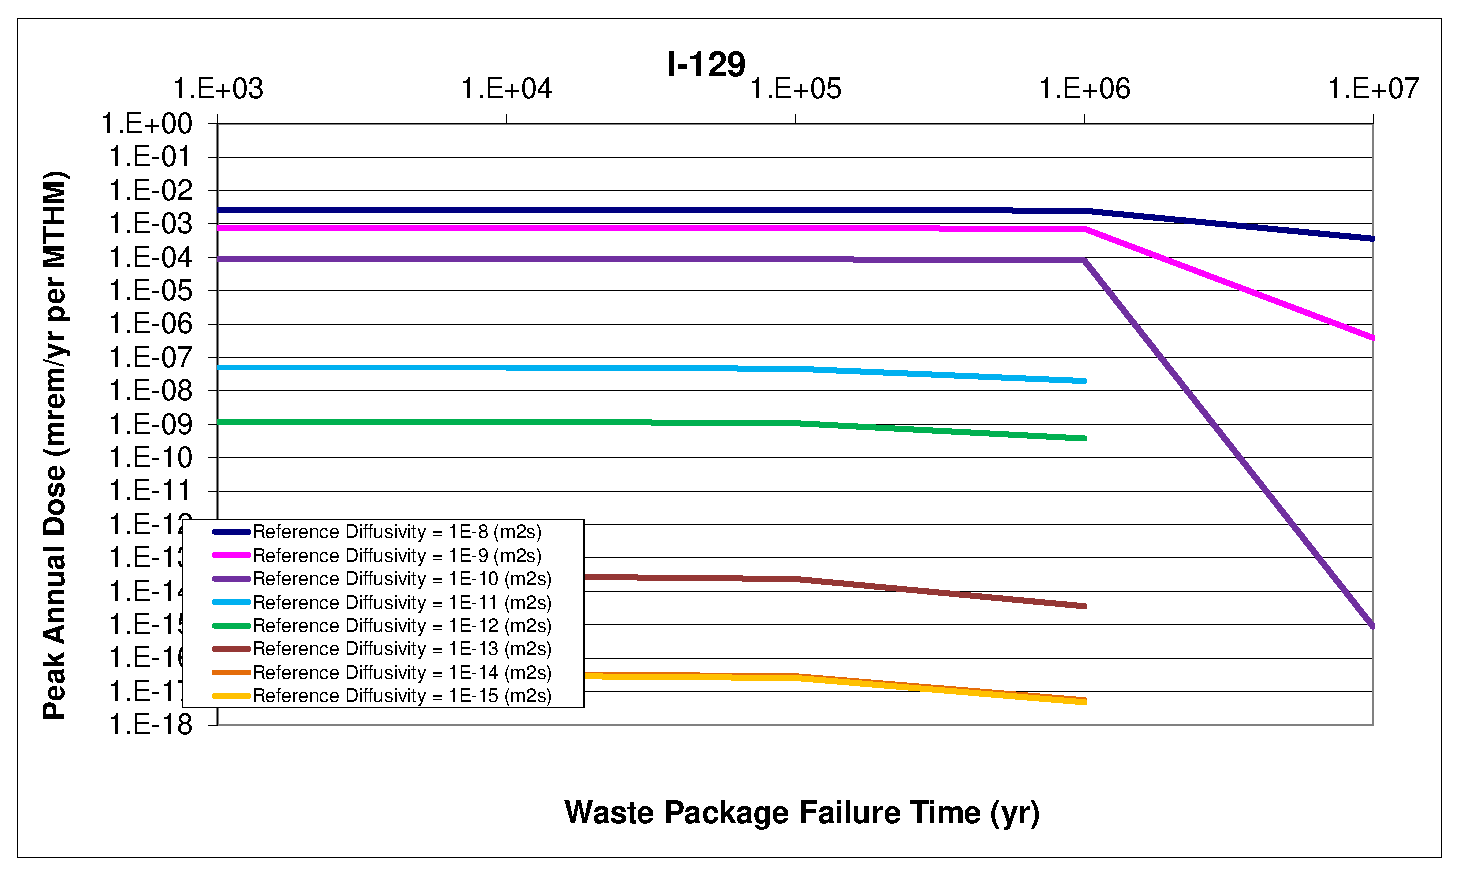
\includegraphics[width=\linewidth]{./chapters/nuclide_sensitivity/clay/WPFailExtended/I-129-WPFail.eps}
    \caption{$^{129}I$ waste package failure time sensitivity. }
    \label{fig:WPFailI129}

  \end{minipage}
\end{figure}
\begin{figure}[ht]
  \begin{minipage}[b]{0.45\linewidth}

    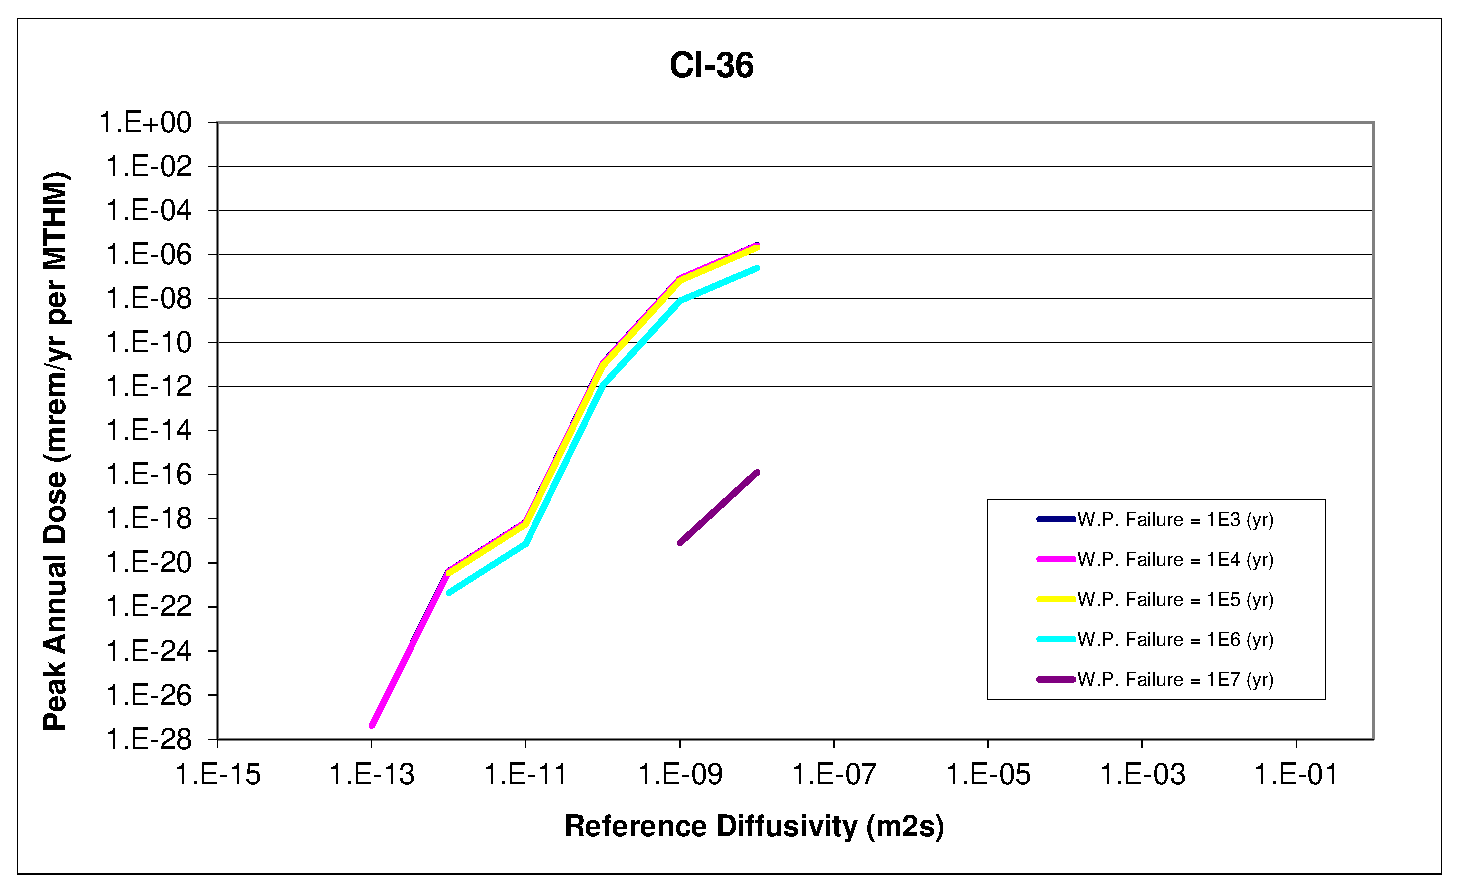
\includegraphics[width=\linewidth]{./chapters/nuclide_sensitivity/clay/WPFailExtended/Cl-36.eps}
    \caption{$^{36}Cl$ waste package failure time sensitivity. }
    \label{fig:WPFailCl36}

  \end{minipage}
  \hspace{0.05\linewidth}
  \begin{minipage}[b]{0.45\linewidth}

    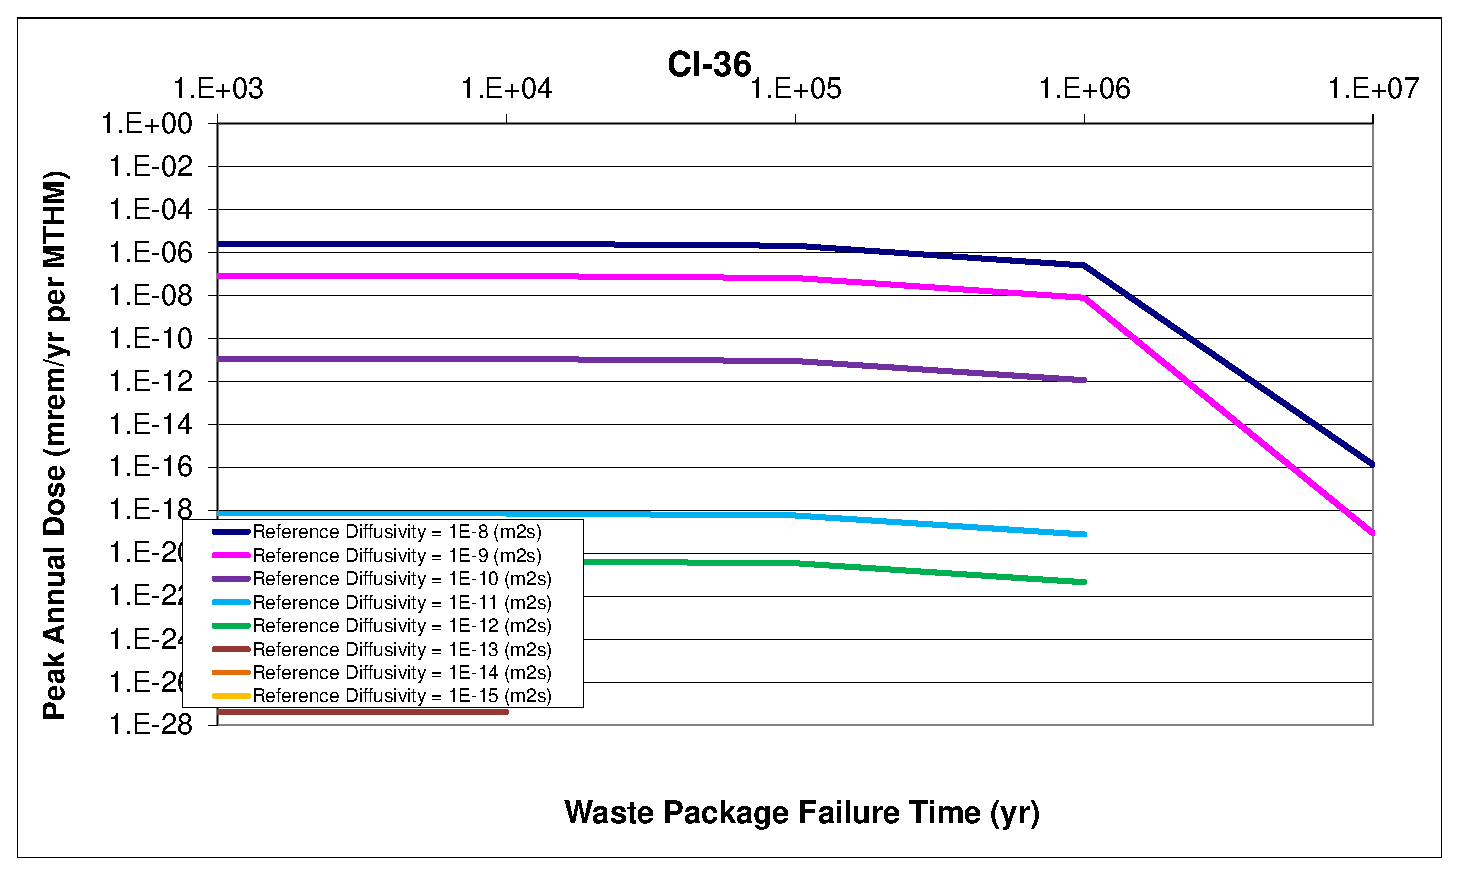
\includegraphics[width=\linewidth]{./chapters/nuclide_sensitivity/clay/WPFailExtended/Cl-36-WPFail.eps}
    \caption{$^{36}Cl$ waste package failure time sensitivity. }
    \label{fig:WPFailPuDaughters}

  \end{minipage}
\end{figure}


\begin{figure}[ht!]
  \centering
  \begin{minipage}[b]{0.45\linewidth}

    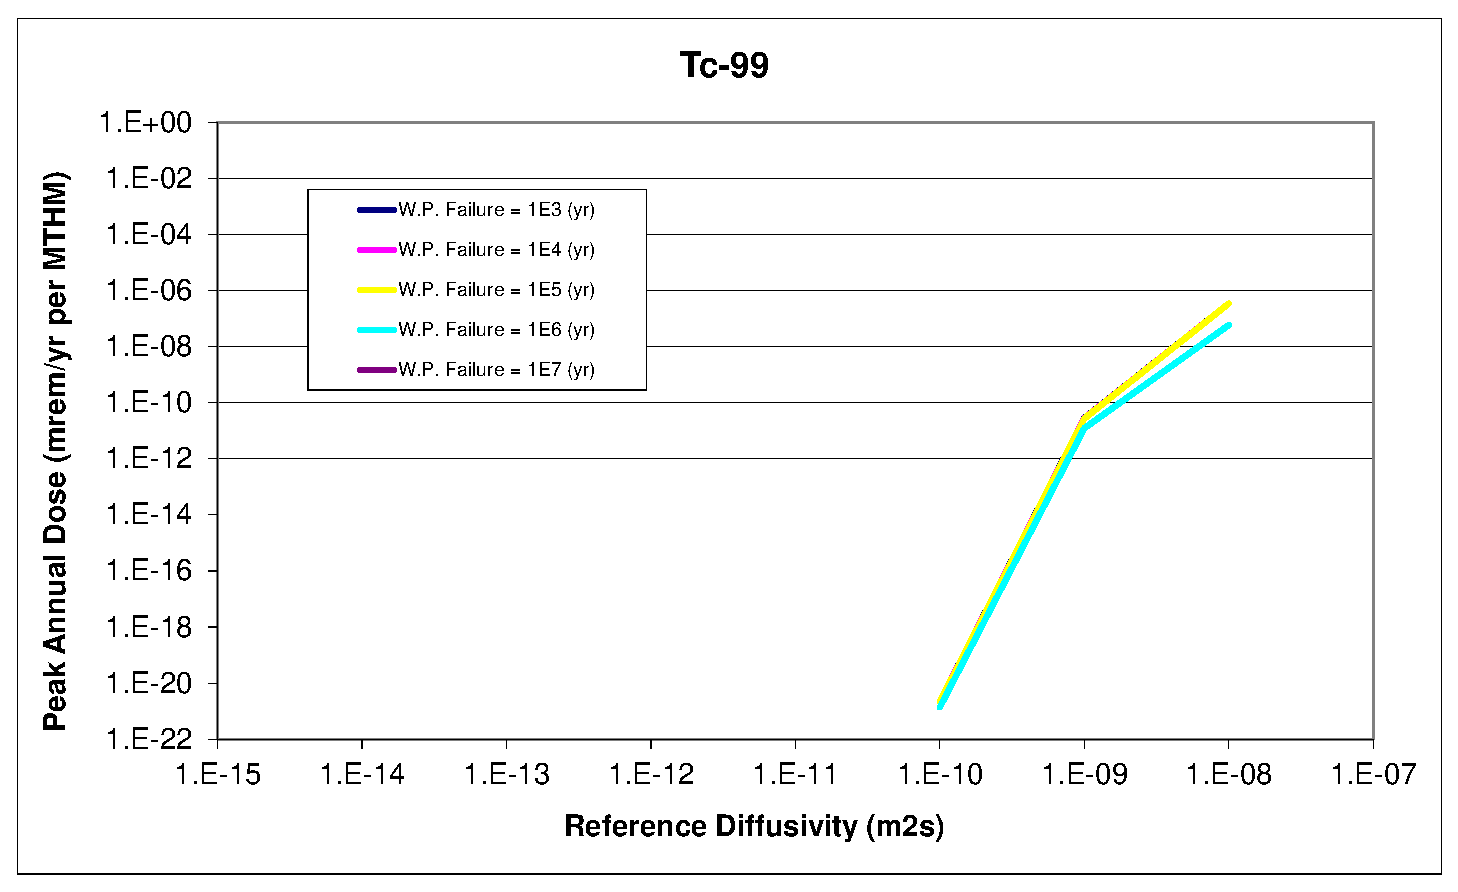
\includegraphics[width=\linewidth]{./chapters/nuclide_sensitivity/clay/WPFailExtended/Tc-99.eps}
    \caption{$^{99}Tc$ waste package failure time sensitivity. }
    \label{fig:WPFailTc99}

  \end{minipage}
  \hspace{0.05\linewidth}
  \begin{minipage}[b]{0.45\linewidth}

    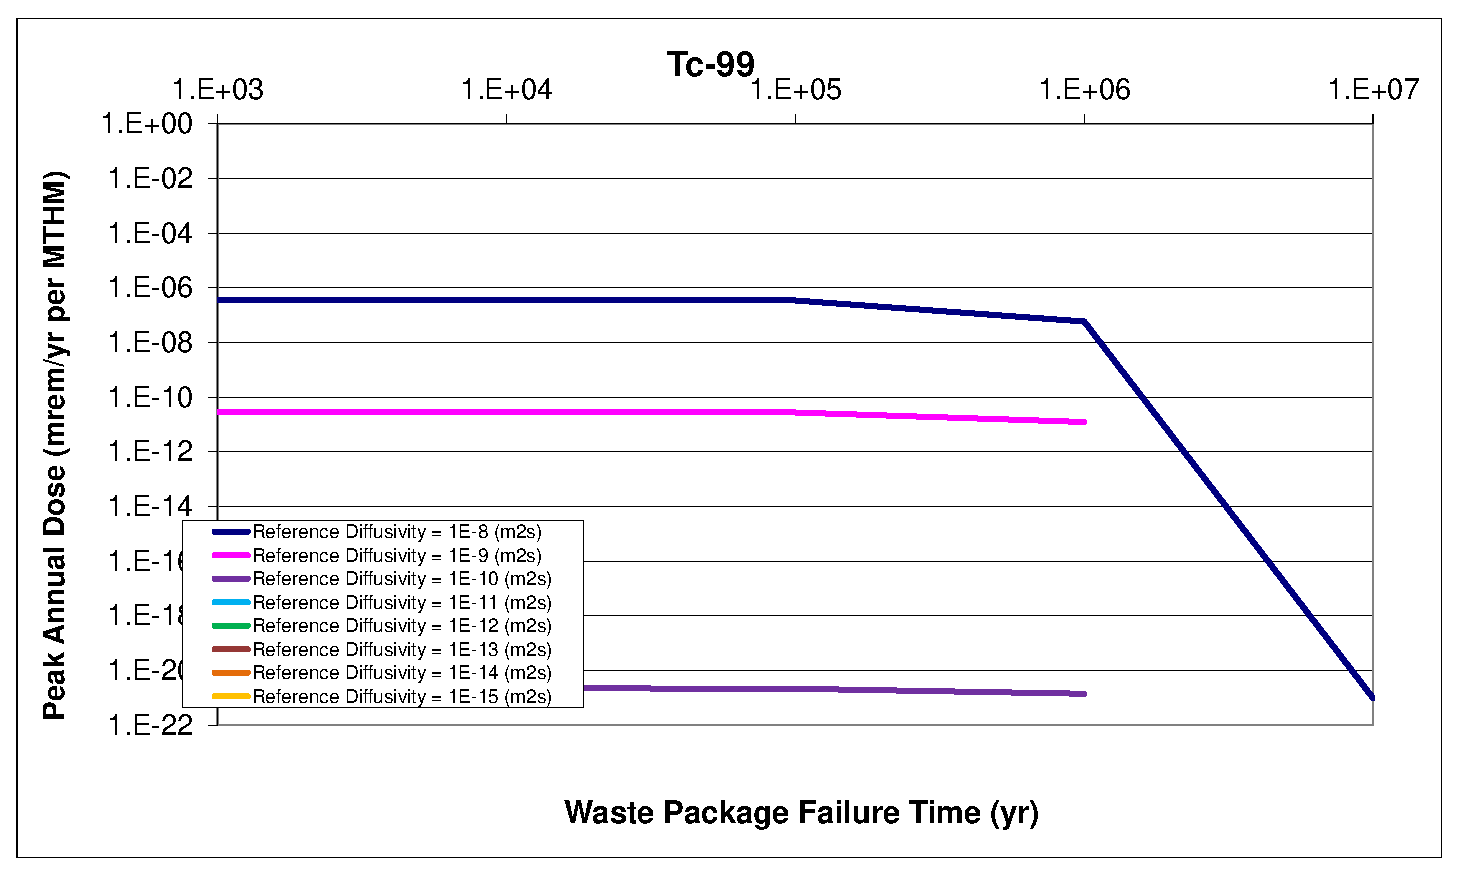
\includegraphics[width=\linewidth]{./chapters/nuclide_sensitivity/clay/WPFailExtended/Tc-99-WPFail.eps}
    \caption{$^{99}Tc$ waste package failure time sensitivity. }
    \label{fig:WPFailTc99}

  \end{minipage}
\end{figure}
\begin{figure}[ht]
  \begin{minipage}[b]{0.45\linewidth}

    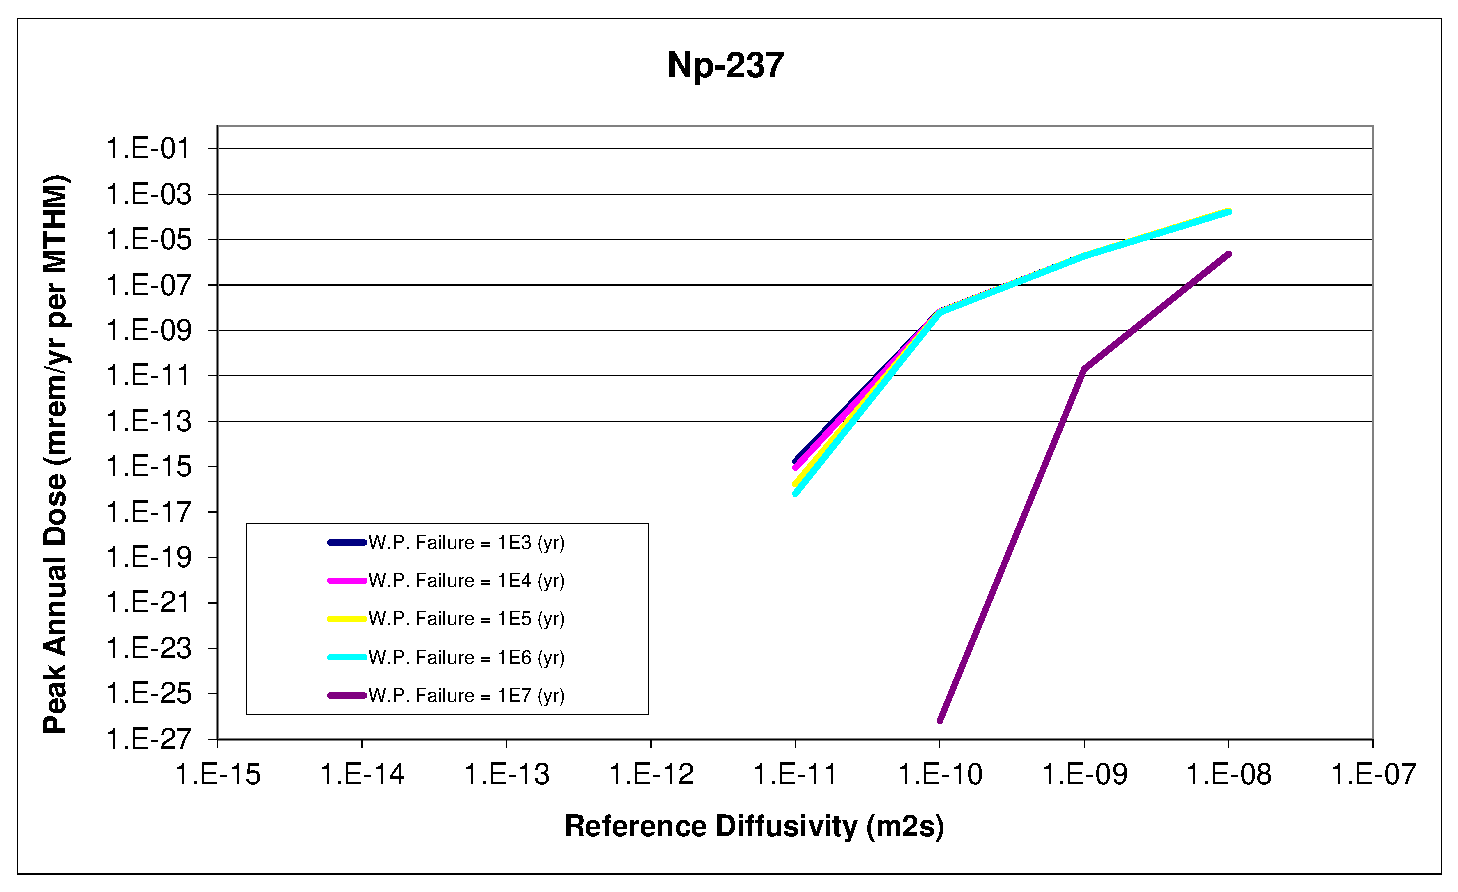
\includegraphics[width=\linewidth]{./chapters/nuclide_sensitivity/clay/WPFailExtended/Np-237.eps}
    \caption{$^{237}Np$ waste package failure time sensitivity. }
    \label{fig:WPFailNp237}

  \end{minipage}
  \hspace{0.05\linewidth}
  \begin{minipage}[b]{0.45\linewidth}

    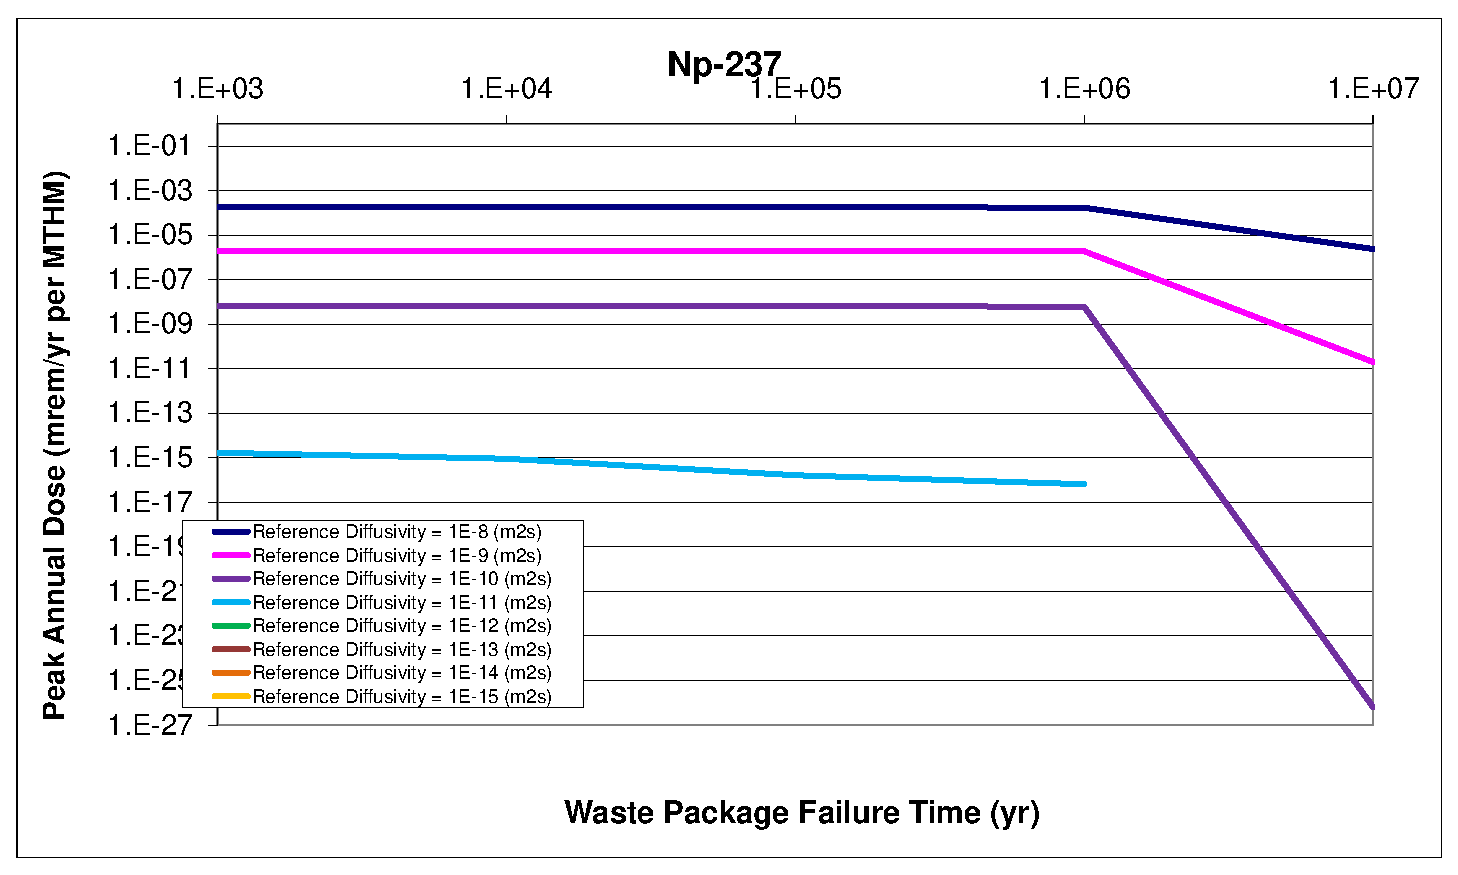
\includegraphics[width=\linewidth]{./chapters/nuclide_sensitivity/clay/WPFailExtended/Np-237-WPFail.eps}
    \caption{$^{237}Np$ waste package failure time sensitivity. }
    \label{fig:WPFailPuDaughters}

  \end{minipage}
\end{figure}

\clearpage



\FloatBarrier
